\documentclass[12pt,twoside,letterpaper]{article}

\newcommand{\reporttitle}{Distributed Learning and Control of Cooperative Quadrotor Load Transportation}
\newcommand{\reportauthorOne}{Gao Yichao}
\newcommand{\cidOne}{A0298755E}
% \newcommand{\reportauthorTwo}{Student 2}
% \newcommand{\cidTwo}{your id number}
% \newcommand{\reporttype}{Coursework}
% \bibliographystyle{plain}

% include files that load packages and define macros
%%%%%%%%%%%%%%%%%%%%%%%%%%%%%%%%%%%%%%%%%
% University Assignment Title Page 
% LaTeX Template
% Version 1.0 (27/12/12)
%
% This template has been downloaded from:
% http://www.LaTeXTemplates.com
%
% Original author:
% WikiBooks (http://en.wikibooks.org/wiki/LaTeX/Title_Creation)
%
% License:
% CC BY-NC-SA 3.0 (http://creativecommons.org/licenses/by-nc-sa/3.0/)
% 
% Instructions for using this template:
% This title page is capable of being compiled as is. This is not useful for 
% including it in another document. To do this, you have two options: 
%
% 1) Copy/paste everything between \begin{document} and \end{document} 
% starting at \begin{titlepage} and paste this into another LaTeX file where you 
% want your title page.
% OR
% 2) Remove everything outside the \begin{titlepage} and \end{titlepage} and 
% move this file to the same directory as the LaTeX file you wish to add it to. 
% Then add \input{./title_page_1.tex} to your LaTeX file where you want your
% title page.
%
%----------------------------------------------------------------------------------------
%	PACKAGES AND OTHER DOCUMENT CONFIGURATIONS
%----------------------------------------------------------------------------------------
\usepackage{setspace}
% \usepackage{titlesec}
\usepackage{lipsum} % for placeholder text
\usepackage{ragged2e}
\usepackage{ifxetex}
\usepackage{textpos}
% \usepackage{natbib}
\usepackage{kpfonts}
\usepackage[letterpaper,hmargin=2.8cm,vmargin=2.0cm,includeheadfoot]{geometry}
\usepackage{ifxetex}
\usepackage{stackengine}
\usepackage{tabularx,longtable,multirow,subfigure,caption}%hangcaption
% \usepackage{fncylab} %formatting of labels
\usepackage{parskip}
\usepackage{fancyhdr}
\usepackage{color}
\usepackage[tight,ugly]{units}
\usepackage{url}
\usepackage{float}
\usepackage[english]{babel}
\usepackage{amsmath}
\usepackage{graphicx}
\usepackage{subcaption}
% \usepackage{subfig}
\usepackage[colorinlistoftodos]{todonotes}
\usepackage{dsfont}
\usepackage{epstopdf} % automatically replace .eps with .pdf in graphics
% \usepackage{natbib}
 

\usepackage{backref}
\usepackage{array}
\usepackage{latexsym}
\usepackage{etoolbox}

\usepackage{enumerate} % for numbering with [a)] format 

\usepackage{listings}
\usepackage{xcolor}

% MATLAB code style
\lstset{
    language=Matlab,                     % Set language to MATLAB
    basicstyle=\ttfamily\footnotesize,   % Set font and size
    keywordstyle=\color{blue},           % Keywords in blue
    stringstyle=\color{red},             % Strings in red
    commentstyle=\color{green!50!black}, % Comments in green
    numbers=left,                        % Line numbers on the left
    numberstyle=\tiny\color{gray},       % Line numbers styling
    stepnumber=1,                        % Step between line numbers
    numbersep=5pt,                       % Space between numbers and code
    backgroundcolor=\color{gray!10},     % Light gray background
    frame=single,                        % Frame around the code
    breaklines=true,                     % Enable line breaking
    breakatwhitespace=true,              % Break lines only at whitespace
    tabsize=4                            % Set tab size
}

\ifxetex
\usepackage{fontspec}
\setmainfont[Scale=.8]{OpenDyslexic-Regular}
\else
\usepackage[pdftex,pagebackref,hypertexnames=false,colorlinks]{hyperref} % provide links in pdf
% \hypersetup{pdftitle={},
%   pdfsubject={}, 
%   pdfauthor={\reportauthorOne},
%   pdfkeywords={}, 
%   pdfstartview=FitH,
%   pdfpagemode={UseOutlines},% None, FullScreen, UseOutlines
%   bookmarksnumbered=true, bookmarksopen=true, colorlinks,
%     citecolor=black,%
%     filecolor=black,%
%     linkcolor=black,%
%     urlcolor=black}
% \usepackage[all]{hypcap}
\usepackage{arydshln}
\hypersetup{
    pdftitle={},
    pdfsubject={}, 
    pdfauthor={\reportauthorOne},
    pdfkeywords={}, 
    pdfstartview=FitH,
    pdfpagemode={UseOutlines}, % None, FullScreen, UseOutlines
    bookmarksnumbered=true, 
    bookmarksopen=true, 
    colorlinks=false,          % 链接不着色,仅在 PDF 中显示框
    citecolor=black,%
    filecolor=black,%
    linkcolor=black,%
    urlcolor=black,
    % pdfborder={0 0 1},         % PDF 中显示小框,宽度为1
}
\usepackage[all]{hypcap}
\fi

\usepackage{tcolorbox}

% various theorems
\usepackage{ntheorem}
\theoremstyle{break}
\newtheorem{lemma}{Lemma}
\newtheorem{theorem}{Theorem}
\newtheorem{remark}{Remark}
\newtheorem{definition}{Definition}
\newtheorem{proof}{Proof}

% example-environment
\newenvironment{example}[1][]
{ 
\vspace{4mm}
\noindent\makebox[\linewidth]{\rule{\hsize}{1.5pt}}
\textbf{Example #1}\\
}
{ 
\noindent\newline\makebox[\linewidth]{\rule{\hsize}{1.0pt}}
}



%\renewcommand{\rmdefault}{pplx} % Palatino
% \renewcommand{\rmdefault}{put} % Utopia

\ifxetex
\else
\renewcommand*{\rmdefault}{bch} % Charter
\renewcommand*{\ttdefault}{cmtt} % Computer Modern Typewriter
%\renewcommand*{\rmdefault}{phv} % Helvetica
%\renewcommand*{\rmdefault}{iwona} % Avant Garde
\fi

\setlength{\parindent}{0em}  % indentation of paragraph

\setlength{\headheight}{14.5pt}
\pagestyle{fancy}
% make the heading left
\fancyhead[EL,OL]{\textit{\leftmark}}
\fancyhead[ER,OR]{}
% make the foot on right
\fancyfoot[ER,OR]{\thepage}%Page no. in the left on
                                %odd pages and on right on even pages
\fancyfoot[OC,EC]{\sffamily }
\renewcommand{\headrulewidth}{0.1pt}
\renewcommand{\footrulewidth}{0.1pt}
\captionsetup{margin=10pt,font=small,labelfont=bf}


%--- chapter heading

\def\@makechapterhead#1{%
  \vspace*{10\p@}%
  {\parindent \z@ \raggedright %\sffamily
        %{\Large \MakeUppercase{\@chapapp} \space \thechapter}
        %\\
        %\hrulefill
        %\par\nobreak
        %\vskip 10\p@
    \interlinepenalty\@M
    \Huge \bfseries 
    \thechapter \space\space #1\par\nobreak
    \vskip 30\p@
  }}

%---chapter heading for \chapter*  
\def\@makeschapterhead#1{%
  \vspace*{10\p@}%
  {\parindent \z@ \raggedright
    \sffamily
    \interlinepenalty\@M
    \Huge \bfseries  
    #1\par\nobreak
    \vskip 30\p@
  }}
  



% %%%%%%%%%%%%% boxit
\def\Beginboxit
   {\par
    \vbox\bgroup
	   \hrule
	   \hbox\bgroup
		  \vrule \kern1.2pt %
		  \vbox\bgroup\kern1.2pt
   }

\def\Endboxit{%
			      \kern1.2pt
		       \egroup
		  \kern1.2pt\vrule
		\egroup
	   \hrule
	 \egroup
   }	

\newenvironment{boxit}{\Beginboxit}{\Endboxit}
\newenvironment{boxit*}{\Beginboxit\hbox to\hsize{}}{\Endboxit}



\allowdisplaybreaks

\makeatletter
\newcounter{elimination@steps}
\newcolumntype{R}[1]{>{\raggedleft\arraybackslash$}p{#1}<{$}}
\def\elimination@num@rights{}
\def\elimination@num@variables{}
\def\elimination@col@width{}
\newenvironment{elimination}[4][0]
{
    \setcounter{elimination@steps}{0}
    \def\elimination@num@rights{#1}
    \def\elimination@num@variables{#2}
    \def\elimination@col@width{#3}
    \renewcommand{\arraystretch}{#4}
    \start@align\@ne\st@rredtrue\m@ne
}
{
    \endalign
    \ignorespacesafterend
}
\newcommand{\eliminationstep}[2]
{
    \ifnum\value{elimination@steps}>0\leadsto\quad\fi
    \left[
        \ifnum\elimination@num@rights>0
            \begin{array}
            {@{}*{\elimination@num@variables}{R{\elimination@col@width}}
            |@{}*{\elimination@num@rights}{R{\elimination@col@width}}}
        \else
            \begin{array}
            {@{}*{\elimination@num@variables}{R{\elimination@col@width}}}
        \fi
            #1
        \end{array}
    \right]
    & 
    \begin{array}{l}
        #2
    \end{array}
    &%                                    moved second & here
    \addtocounter{elimination@steps}{1}
}
\makeatother

%% Fast macro for column vectors
\makeatletter  
\def\colvec#1{\expandafter\colvec@i#1,,,,,,,,,\@nil}
\def\colvec@i#1,#2,#3,#4,#5,#6,#7,#8,#9\@nil{% 
  \ifx$#2$ \begin{bmatrix}#1\end{bmatrix} \else
    \ifx$#3$ \begin{bmatrix}#1\\#2\end{bmatrix} \else
      \ifx$#4$ \begin{bmatrix}#1\\#2\\#3\end{bmatrix}\else
        \ifx$#5$ \begin{bmatrix}#1\\#2\\#3\\#4\end{bmatrix}\else
          \ifx$#6$ \begin{bmatrix}#1\\#2\\#3\\#4\\#5\end{bmatrix}\else
            \ifx$#7$ \begin{bmatrix}#1\\#2\\#3\\#4\\#5\\#6\end{bmatrix}\else
              \ifx$#8$ \begin{bmatrix}#1\\#2\\#3\\#4\\#5\\#6\\#7\end{bmatrix}\else
                 \PackageError{Column Vector}{The vector you tried to write is too big, use bmatrix instead}{Try using the bmatrix environment}
              \fi
            \fi
          \fi
        \fi
      \fi
    \fi
  \fi 
}  
\makeatother

\robustify{\colvec}

%%% Local Variables: 
%%% mode: latex
%%% TeX-master: "notes"
%%% End: 
 % various packages needed for maths etc.
% quick way of adding a figure
\newcommand{\fig}[3]{
 \begin{center}
 \scalebox{#3}{\includegraphics[#2]{#1}}
 \end{center}
}

%\newcommand*{\point}[1]{\vec{\mkern0mu#1}}
\newcommand{\ci}[0]{\perp\!\!\!\!\!\perp} % conditional independence
\newcommand{\point}[1]{{#1}} % points 
\renewcommand{\vec}[1]{{\boldsymbol{{#1}}}} % vector
\newcommand{\mat}[1]{{\boldsymbol{{#1}}}} % matrix
\newcommand{\R}[0]{\mathds{R}} % real numbers
\newcommand{\Z}[0]{\mathds{Z}} % integers
\newcommand{\N}[0]{\mathds{N}} % natural numbers
\newcommand{\nat}[0]{\mathds{N}} % natural numbers
\newcommand{\Q}[0]{\mathds{Q}} % rational numbers
\ifxetex
\newcommand{\C}[0]{\mathds{C}} % complex numbers
\else
\newcommand{\C}[0]{\mathds{C}} % complex numbers
\fi
\newcommand{\tr}[0]{\text{tr}} % trace
\renewcommand{\d}[0]{\mathrm{d}} % total derivative
\newcommand{\inv}{^{-1}} % inverse
\newcommand{\id}{\mathrm{id}} % identity mapping
\renewcommand{\dim}{\mathrm{dim}} % dimension
\newcommand{\rank}[0]{\mathrm{rk}} % rank
\newcommand{\determ}[1]{\mathrm{det}(#1)} % determinant
\newcommand{\scp}[2]{\langle #1 , #2 \rangle}
\newcommand{\kernel}[0]{\mathrm{ker}} % kernel/nullspace
\newcommand{\img}[0]{\mathrm{Im}} % image
\newcommand{\idx}[1]{{(#1)}}
\DeclareMathOperator*{\diag}{diag}
\newcommand{\E}{\mathds{E}} % expectation
\newcommand{\var}{\mathds{V}} % variance
\newcommand{\gauss}[2]{\mathcal{N}\big(#1,\,#2\big)} % gaussian distribution N(.,.)
\newcommand{\gaussx}[3]{\mathcal{N}\big(#1\,|\,#2,\,#3\big)} % gaussian distribution N(.|.,.)
\newcommand{\gaussBig}[2]{\mathcal{N}\left(#1,\,#2\right)} % see above, but with brackets that adjust to the height of the arguments
\newcommand{\gaussxBig}[3]{\mathcal{N}\left(#1\,|\,#2,\,#3\right)} % see above, but with brackets that adjust to the height of the arguments
\DeclareMathOperator{\cov}{Cov} % covariance (matrix) 
\ifxetex
\renewcommand{\T}[0]{^\top} % transpose
\else
\newcommand{\T}[0]{^\top}
\fi
% matrix determinant
\newcommand{\matdet}[1]{
\left|
\begin{matrix}
#1
\end{matrix}
\right|
}



%%% various color definitions
\definecolor{darkgreen}{rgb}{0,0.6,0}

\newcommand{\blue}[1]{{\color{blue}#1}}
\newcommand{\red}[1]{{\color{red}#1}}
\newcommand{\green}[1]{{\color{darkgreen}#1}}
\newcommand{\orange}[1]{{\color{orange}#1}}
\newcommand{\magenta}[1]{{\color{magenta}#1}}
\newcommand{\cyan}[1]{{\color{cyan}#1}}


% redefine emph
% \renewcommand{\emph}[1]{\blue{\bf{#1}}}

% place a colored box around a character
\gdef\colchar#1#2{%
  \tikz[baseline]{%
  \node[anchor=base,inner sep=2pt,outer sep=0pt,fill = #2!20] {#1};
    }%
}%
 % short-hand notation and macros


%%%%%%%%%%%%%%%%%%%%%%%%%%%%

\begin{document}
% front page
% Last modification: 2016-09-29 (Marc Deisenroth)
% Modification for UW: 2017-05-22 (jphickey)
% Modification for NUS: 2024-08-22 (yuxiangxiao)
\begin{titlepage}

\newcommand{\HRule}{\rule{\linewidth}{0.5mm}} % Defines a new command for the horizontal lines, change thickness here


%----------------------------------------------------------------------------------------
%	LOGO SECTION
%----------------------------------------------------------------------------------------



\begin{center} % Center remainder of the page

%----------------------------------------------------------------------------------------
%	HEADING SECTIONS
%----------------------------------------------------------------------------------------


\includegraphics[width = 10cm]{./figures/nus}\\[1.0cm] 
\textbf{\textsc{\Large EE5003 - Project Report}}\\[1.0cm] 
\textsc{\Large National University of Singapore}\\[0.5cm] 
\textsc{\large Department of Electrical \& Computer Engineering}\\[0.95cm] 

%----------------------------------------------------------------------------------------
%	TITLE SECTION
%----------------------------------------------------------------------------------------

\HRule \\[0.4cm]
{ \LARGE \bfseries \reporttitle}\\ % Title of your document
\HRule \\[1.5cm]
\end{center}
%----------------------------------------------------------------------------------------
%	AUTHOR SECTION
%----------------------------------------------------------------------------------------

%\begin{minipage}{0.4\hsize}
\begin{center}
   by:
\end{center}
\begin{flushleft} \large
% \textit{Author:}
\begin{center}
    \reportauthorOne~(ID: \cidOne)\\ % Your name
\end{center}
\begin{center}
    yichao\_gao@u.nus.edu
\end{center}

% \reportauthorTwo~(ID: \cidTwo) % Your name
\end{flushleft}
% \vspace{3cm}
\vspace{0.5cm}
\begin{center}\large
    Supervisor: Dr. Zhao Lin
\end{center}
\begin{center}\large
    Examiner: Prof. Ge Shuzhi Sam
\end{center}
\makeatletter
\vspace{1cm}
\begin{center}
    April~~2025
\end{center}
% \@date 

\vfill % Fill the rest of the page with whitespace





\end{titlepage}



\begin{center}
    \section*{Abstract}
\end{center}
\addcontentsline{toc}{section}{Abstract}
 Multi-lift aerial transportation, in which multiple quadrotors collaboratively carry a common payload via cables, has been extensively explored to enhance load-carrying capacity and increase system redundancy. However, existing simulation platforms and software pipelines have not matured to meet the complex requirements of such tasks. In particular, there is currently no comprehensive simulator that seamlessly integrates all the necessary components for multi-lift research: Isaac Sim for high-fidelity physics, PX4 for low-level flight control, ROS for communication and orchestration, and self-defined reinforcement learning (RL) algorithms for high-level policy training. The absence of such toolchain not only limits the ability to test advanced control and learning strategies but also makes it difficult to bridge the gap between simulated performance and real-world behavior.

In this work, we develop a high-fidelity software-in-the-loop (SITL) framework for multi-lift aerial transportation that addresses these challenges. Building on Isaac Sim’s Temporal Gauss–Seidel (TGS) solver, we introduce a mass–spring–damper (MSD) cable model capable of handling highly stiff tethers under real-time constraints. This ensures a stable and accurate representation of cable dynamics in various cooperative load-sharing scenarios. Meanwhile, we integrate PX4-based flight controllers and ROS\,2 communication layers to achieve minimal-latency data exchange and synchronized state estimation. A geometric controller with decoupled yaw regulation is implemented as a robust low-level flight-control strategy, while the system architecture accommodates self-defined RL modules for distributed learning of high-level control policies.

Through extensive tests—ranging from basic cable-dynamics validation to cooperative trajectory tracking with multiple UAVs—the proposed platform demonstrates reliable real-time operation and consistent tracking accuracy. In addition, the design naturally accommodates wind disturbances and varying payload conditions, thus expanding the scope of scenarios that can be evaluated. While this framework lays a strong foundation for the simulation of multi-lift systems, future efforts will focus on refining aerodynamic models (e.g., rotor wash, turbulence) and incorporating hardware-in-the-loop components for more seamless transitions to physical flight tests. Overall, the presented SITL environment provides a long-awaited solution for validating advanced learning and control algorithms in multi-lift tasks and paves the way for safer, more efficient aerial cargo transport.

\newpage

\begin{center}
    \section*{Acknowledgement}
\end{center}
\addcontentsline{toc}{section}{Acknowledgement}
My time as a Master’s student at the NUS - ECE has been both a challenging and enriching experience. Over the course of this journey, I’ve had the privilege to engage in academic research, explore new areas within engineering, and develop both personally and intellectually. This report is a reflection of that journey, which is shaped not only by my efforts but also by the generous support, guidance, and encouragement I’ve received from many along the way.

Foremost among those I wish to acknowledge is my supervisor, Dr. Zhao Lin, whose exceptional mentorship has been profoundly influential throughout my academic journey. Prof. Zhao has provided invaluable guidance that has significantly shaped the direction and depth of my research. His insightful feedback and unwavering support have greatly enriched my understanding of these complex fields and have been instrumental in my academic and personal development.  

I would also like to extend my thanks to Dr. Wang Bingheng for his support in both academic research and coursework. Dr. Wang is a dedicated scholar, whose seriousness and unwavering commitment to scientific inquiry have profoundly influenced me. 

In addition, I would like to express my gratitude for the support of many researchers and friends, including but not limited to Dr. He Lei, Sun Tianchen, Sima Kuankuan, Huang Rui and Chen Xin. Their advice and insightful perspectives on academic topics have significantly contributed to my progress in research. Special thanks go to Tang Longbin, for making both coursework and research endeavors productive and enjoyable.

Lastly, I extend my deepest gratitude to my family—my parents and my sister—for their unwavering love and support. Their encouragement and belief in me have been my foundation throughout this journey, giving me the strength and confidence to pursue my goals.

\newpage


\begin{center}
    \section*{Declaration}
\end{center}
\addcontentsline{toc}{section}{Declaration}

\vspace{2cm}

\begin{center}
    \begin{minipage}{0.8\textwidth}
        \centering
        \doublespacing
        \justifying
        \large
        \begin{center}
            I hereby declare that this report is my original work and it has been written by me in its entirety. 
            
            I have duly acknowledged all the sources of information which have been used in the report.
        \end{center}
    \end{minipage}
    \vspace{2cm}  

    \begin{figure}[H]
    \centering
    \begin{minipage}{0.5\textwidth}
        \centering
        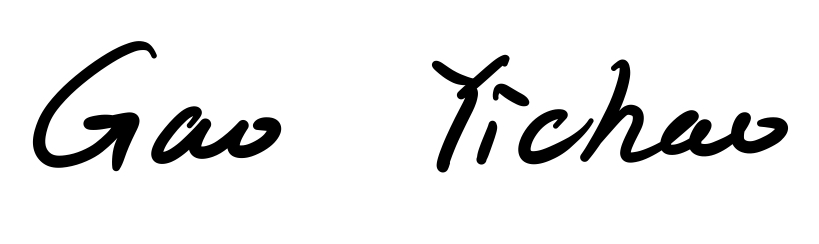
\includegraphics[width=\linewidth]{figures/sign.jpeg}
        \vspace{0.5cm}
        \caption*{April 1st, 2025}
        \label{fig:minipage-example}
    \end{minipage}
\end{figure}

    
\end{center}
\newpage


%%%%%%%%%%%%%%%%%%%%%%%%%%% table of content
%If a table of content is needed, simply uncomment the following lines
\begin{center}
\tableofcontents
\end{center}
\newpage

\begin{center}
    \listoffigures
\end{center}
\addcontentsline{toc}{section}{List of Figures}


\newpage

%%%%%%%%%%%%%%%%%%%%%%%%%%%% Main document
% \section*{Note:}
% \emph{This document is intended to provide a sample structure for the reports in ME303 at the University of Waterloo. }

\section{Introduction}
Aerial transportation using multiple quadrotors has garnered substantial interest in the robotics and unmanned aerial vehicle (UAV) communities due to its enhanced load-carrying capacity and improved robustness compared to single-vehicle systems. By attaching the payload via lightweight cables, multi-lift configurations can accommodate large and potentially heavy loads. However, these systems are inherently complex: each quadrotor’s motion is constrained by cable length when taut, and dynamic coupling through the cables introduces intricate force interactions among vehicles and the load. Additionally, the system exhibits hybrid dynamics owing to transitions between slack and taut states, rendering motion planning and control significantly more challenging. Achieving safe and effective coordination requires addressing cable slack avoidance, maintaining inter-vehicle distances, managing control limits, and ensuring scalability with an increasing number of UAVs.

\begin{figure}[H]
    \centering
    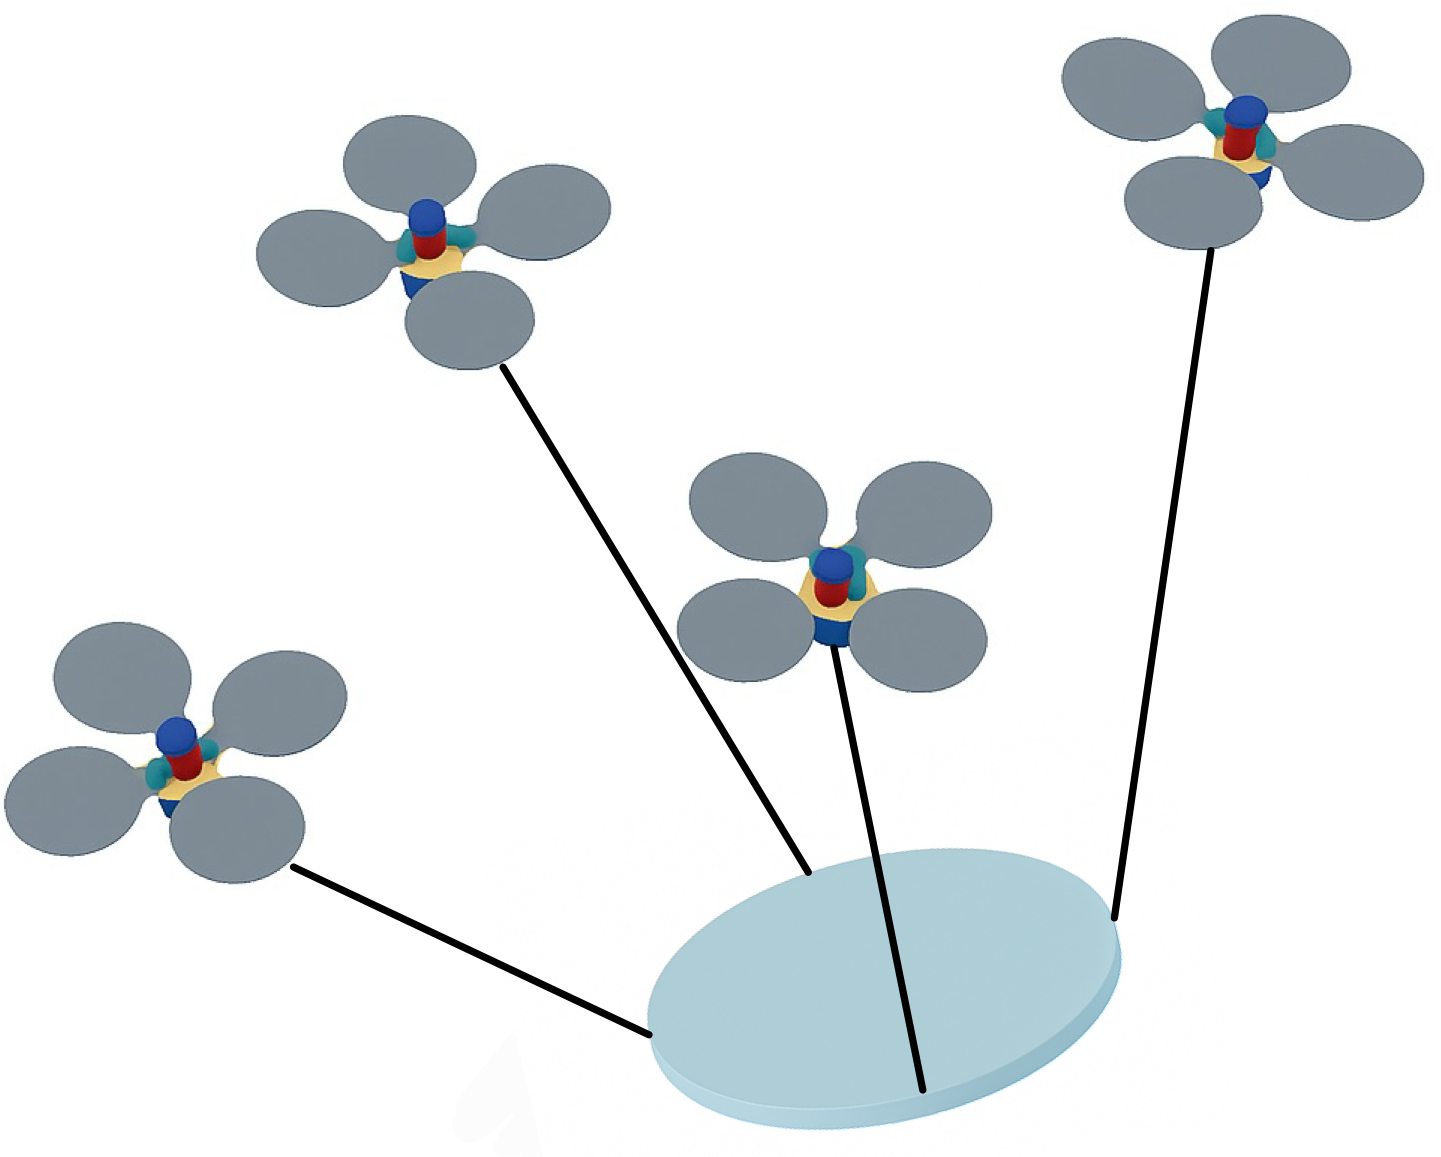
\includegraphics[width=0.5\linewidth]{figures/Multilift.png}
    \caption{Illustration of Multilift Problems}
    \label{multilift}
\end{figure}

Early investigations into multi-lift aerial transport often simplified the payload as a point mass, wherein cable tensions were treated as external disturbances acting on the quadrotors \cite{Geo_point},\cite{2018point}. Although these models facilitated initial theoretical and experimental studies, they limited achievable maneuvers to near-quasistatic or slow trajectories. Subsequent research endeavored to capture the dynamic coupling between quadrotors and payload more accurately. In particular, \cite{2014Geo} introduced a geometric control framework that explicitly accounts for the payload’s dynamics as a point mass. Further enhancements included modeling the payload as a full six-degrees-of-freedom rigid body, enabling higher-fidelity control but demanding at least three quadrotors for complete attitude and position regulation \cite{sreenath2013dynamics},\cite{lee2017geometric}.

More recent work has pushed toward agile and robust control of cable-suspended loads. Sun \cite{sun2025agilecooperativeaerialmanipulation} proposed a model predictive control (MPC)-based solution for high-acceleration payload transport without onboard sensors, addressing dynamic coupling and load uncertainties. However, the reliance on carefully tuned MPC parameters remained a practical challenge. Wang \cite{wang2025safeagiletransportationcablesuspended} introduced a distributed, learning-based approach that enables real-time trajectory planning and control in cluttered environments, though this method simplifies the payload to a point mass and neglects its full dynamic behavior.

Auto-Multilift \cite{multilift} offers a distributed closed-loop learning framework to automatically adapt MPC hyperparameters for multi-lift systems. At its core, a Distributed Sensitivity Propagation (DSP) algorithm is employed to compute closed-loop state sensitivities in parallel, informing a distributed policy gradient method that trains deep neural networks using tracking error feedback. This approach leverages the Safe-PDP-based MPC gradient solver, improving scalability and ensuring robust trajectory tracking compared to open-loop MPC parameter tuning.

To investigate the stability and practical feasibility of Auto-Multilift, a high-fidelity simulator that accurately captures multi-lift aerial systems is essential. Hence, this work extends Isaac Sim and Pegasus \cite{pegasus} with refined quadrotor dynamics and flexible cable modeling. In particular, the cable model is formulated as a mass-spring-damper (MSD) system with multiple joints, capturing the high stiffness required in real-world tethering scenarios. Traditional simulators, such as Gazebo and MuJoCo, often struggle to simulate such highly stiff, multi-joint connections in real time. By leveraging the high computational power and stability of PhysX through the fast TGS (Temporal Gauss-Seidel) numerical solver, Isaac Sim can now operate in real time while accurately reproducing the physics of complex cable dynamics.

A ROS-based communication pipeline is also developed to facilitate software-in-the-loop (SITL) simulation with PX4, ensuring precise time synchronization and reliable exchange of states between the flight controller, ground station, and simulation environment. Additionally, a geometric controller with decoupled yaw-axis regulation is integrated as the low-level controller for individual UAV stabilization and trajectory tracking.

\textbf{The main contributions of this work are as follows:} \begin{enumerate} 
\item \textbf{Development of a high-fidelity simulation environment for multi-lift aerial systems}: This environment, built upon Isaac Sim and Pegasus, incorporates improved quadrotor and cable dynamics through an MSD model with multiple joints. 
\item \textbf{Design of a ROS-based SITL pipeline}: A specialized communication framework is implemented to ensure consistent time synchronization and robust state exchange among PX4, the ground control station, and the simulator. 
\item \textbf{Integration of a geometric low-level controller}: A geometric controller with decoupled yaw-axis dynamics is presented, enabling precise single-UAV stabilization and control in multi-lift operations. 
\end{enumerate}


\newpage


% \section{Model of Multilift Systems}

% \newpage


\section{Simulator Design}
\subsection{Quadrotor Dynamics}
 In this subsection, we present a comprehensive overview of the quadrotor’s translational and rotational equations of motion. We then highlight the improvements introduced in the Pegasus Simulator, which result in a more accurate representation of quadrotor dynamics. Notably, all rotational quantities are expressed on the special orthogonal group 
$\mathrm{SO}(3)$, ensuring a globally valid description of the quadrotor’s attitude.

Define an inertial frame $\{\mathcal{I}\}$ and a body frame $\{\mathcal{B}\}$ fixed to the quadrotor’s center of mass. Let 
$\mathbf{p} \in \mathbb{R}^3$
denote the position of the quadrotor’s center of mass expressed in the inertial frame, and let
$\mathbf{R} \in \mathrm{SO}(3)$
describe the orientation of the body frame with respect to the inertial frame. The time derivative $\dot{\mathbf{p}} \in \mathbb{R}^3$ denotes the linear velocity, and the angular velocity in the body frame is 
$\boldsymbol{\Omega} \in \mathbb{R}^3.$
The vehicle has mass $m>0$, a (typically diagonal) moment of inertia matrix $\mathbf{I}\in \mathbb{R}^{3\times 3}$, and experiences gravity $g>0$ acting in the $-z$ direction of the inertial frame.

\paragraph{Translational Dynamics.} 
Newton’s second law gives the translational dynamics of the quadrotor’s center of mass. The primary external forces are gravity and the total thrust generated by the four rotors. Let $T \ge 0$ denote the total thrust, which acts along the body’s $z$-axis. Transformed into the inertial frame, the thrust vector becomes $\mathbf{R}\,\mathbf{e}_3\,T$, where $\mathbf{e}_3 = [\,0\;\;0\;\;1\,]^\top$. Consequently, the translational dynamics are
\begin{equation}
    m\,\ddot{\mathbf{p}} \;=\; -m\,g\,\mathbf{e}_3 \;+\; T\,\mathbf{R}\,\mathbf{e}_3.
    \label{eq:translational_dynamics}
\end{equation}

\paragraph{Rotational Kinematics.} 
The evolution of the orientation matrix $\mathbf{R}$ is governed by
\begin{equation}
    \dot{\mathbf{R}} \;=\; \mathbf{R}\,\widehat{\boldsymbol{\Omega}},
    \label{eq:rotational_kinematics}
\end{equation}
where $\widehat{\boldsymbol{\Omega}}$ is the skew-symmetric matrix associated with the cross product in $\mathbb{R}^3$, namely
\begin{equation}
    \widehat{\boldsymbol{\Omega}} 
    \;=\;
    \begin{bmatrix}
    0 & -\Omega_3 & \Omega_2 \\
    \Omega_3 & 0 & -\Omega_1 \\
    -\Omega_2 & \Omega_1 & 0
    \end{bmatrix}.
\end{equation}

\paragraph{Rotational Dynamics.} 
The rotational motion obeys Euler’s equation in the body frame:
\begin{equation}
    \mathbf{I}\,\dot{\boldsymbol{\Omega}} 
    \;+\;
    \boldsymbol{\Omega} \times \bigl(\mathbf{I}\,\boldsymbol{\Omega}\bigr)
    \;=\;
    \boldsymbol{\tau},
    \label{eq:rotational_dynamics}
\end{equation}
where $\boldsymbol{\tau} \in \mathbb{R}^3$ is the net torque in the body frame. For a symmetric quadrotor, $\mathbf{I} = \mathrm{diag}(I_x, I_y, I_z)$ and the cross-product terms simplify, but we retain the general form in Eq.~\eqref{eq:rotational_dynamics} for completeness.

\paragraph{Thrust Allocation.} 
Each rotor generates a thrust force proportional to the square of its rotational speed. Let $\omega_i$ be the angular speed of rotor $i$, and let $b>0$ denote the thrust coefficient. Then the thrust of rotor $i$ is 
\begin{equation}
f_i = b\,\omega_i^2, 
\quad i=1,\dots,4.
\end{equation}
Hence the total thrust $T$ is
\begin{equation}
    T \;=\; \sum_{i=1}^{4} f_i 
    \;=\; b\bigl(\omega_1^2 + \omega_2^2 + \omega_3^2 + \omega_4^2 \bigr).
    \label{eq:total_thrust}
\end{equation}
Additionally, each rotor creates a torque about its own axis, often modeled as 
\begin{equation}
\tau_{\mathrm{drag},i} = d\,\omega_i^2,
\end{equation}
where $d>0$ is the drag coefficient. The \emph{net} torque in the body frame arises from the combination of torques due to (1) the lateral distance of each rotor thrust from the center of mass, and (2) the drag torques induced by rotor spinning. Labeling the four rotors such that $\omega_1$ and $\omega_3$ spin in one direction, and $\omega_2$ and $\omega_4$ spin in the opposite direction, one obtains the commonly used expressions for roll, pitch, and yaw torques:
\begin{equation}
    \tau_{\phi} \;=\; \ell\,b\,(\omega_2^2 - \omega_4^2), 
    \qquad
    \tau_{\theta} \;=\; \ell\,b\,(\omega_3^2 - \omega_1^2), 
    \qquad
    \tau_{\psi} \;=\; d\,(\omega_1^2 - \omega_2^2 + \omega_3^2 - \omega_4^2),
\end{equation}
where $\ell$ is the length of each rotor arm. Stacking these into the vector $\boldsymbol{\tau} = [\,\tau_{\phi}\;\;\tau_{\theta}\;\;\tau_{\psi}\,]^\top$ yields
\begin{equation}
    \boldsymbol{\tau} 
    \;=\;
    \begin{bmatrix}
    \tau_{\phi} \\
    \tau_{\theta} \\
    \tau_{\psi}
    \end{bmatrix}.
\end{equation}

A common approach is to collect the force and torque components into a single control vector
\begin{equation}
    \mathbf{u}
    \;=\;
    \begin{bmatrix}
    T \\[4pt]
    \tau_{\phi} \\[3pt]
    \tau_{\theta} \\[3pt]
    \tau_{\psi}
    \end{bmatrix},
    \quad
    \text{and define}
    \quad
    \boldsymbol{\omega}^2
    \;=\;
    \begin{bmatrix}
    \omega_1^2 \\[4pt]
    \omega_2^2 \\[4pt]
    \omega_3^2 \\[4pt]
    \omega_4^2
    \end{bmatrix}.
\end{equation}
Then,
\begin{equation}
    \mathbf{u} 
    \;=\;
    \begin{bmatrix}
    b & b & b & b \\
    0 & \ell\,b & 0 & -\ell\,b \\
    -\ell\,b & 0 & \ell\,b & 0 \\
    d & -d & d & -d
    \end{bmatrix}
    \,\boldsymbol{\omega}^2,
    \label{eq:allocation_matrix}
\end{equation}
where the $4\times4$ matrix on the right-hand side is referred to as the \emph{allocation matrix}. By inverting or pseudo-inverting this matrix, one can obtain the required rotor speeds (or squared speeds) to achieve a desired thrust and torque vector.

The Pegasus Simulator incorporates detailed quadrotor dynamics within the simulation environment. However, it does not account for wind effects or aerodynamic drag \cite{martin2010true}, which can lead to inaccuracies and contribute to a significant sim-to-real gap. To further reduce this gap, we extend the simulator by incorporating wind disturbances and rolling moments, effectively modeling aerodynamic drag and external disturbances more realistically.

\begin{equation}
    \mathbf{I}\,\dot{\boldsymbol{\Omega}}
    \;+\;
    \boldsymbol{\Omega} \times \bigl(\mathbf{I}\,\boldsymbol{\Omega}\bigr)
    \;=\;
    \boldsymbol{\tau}
    \;+\;
    \boldsymbol{\tau}_{\mathrm{dist}},
    \label{eq:rotational_disturbance}
\end{equation}
where
\begin{equation}
    \boldsymbol{\tau}_{\mathrm{dist}}
    \;=\;
    \bigl[\,
    \tau_{\phi_d}
    \;\;0\;\;0
    \bigr]^\top,
\end{equation}
represents a wind-induced moment acting primarily about the roll axis, $\tau_{\phi_d}\in \mathbb{R}$. 
By modeling both aerodynamic drag and rolling-moment disturbances linearly, the simulator achieves a more realistic approximation of quadrotor flight under varying wind conditions.


\subsection{Cable Modeling}

In this subsection, we introduce the mass--spring--damper (MSD) model to represent the dynamics of a flexible cable. This modeling approach is frequently employed in the simulation of slender mechanical systems under various loading and boundary conditions. The model is constructed by discretizing the cable into a finite number of lumped masses connected by linear or nonlinear springs and dampers.

To outline the derivation, let us assume that the cable is subdivided into \(N\) segments, each of which is characterized by a small mass \(\Delta m\). We denote the displacement of each mass \(i\) at time \(t\) by \(\mathbf{x}_i(t) \in \mathbb{R}^3\). The governing equations arise from applying Newton's second law to each segment, taking into account both the internal elastic and damping forces between adjacent masses.

\begin{figure}[htbp]
  \centering
  \begin{minipage}{0.7\textwidth}
    \centering
    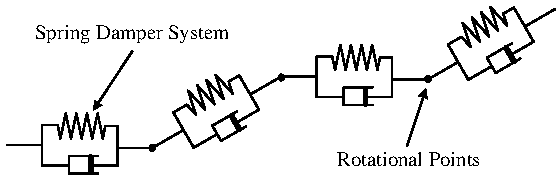
\includegraphics[width=\textwidth]{figures/MSD_model.pdf}
    \caption{Illustration of MSD model for cables.}
    \label{MSD}
  \end{minipage}
\end{figure}


\paragraph{Spring forces}
In the simplest linear case, each segment is modeled using Hooke's law, where the spring force \(\mathbf{F}^{(s)}\) between two adjacent masses \(i\) and \(i+1\) is given by
\begin{equation}
  \mathbf{F}_{i,i+1}^{(s)} 
  = k \Bigl( \|\mathbf{x}_{i+1} - \mathbf{x}_i\| - \ell_0 \Bigr)\,
    \hat{\mathbf{r}}_{i,i+1},
  \label{eq:spring_force}
\end{equation}
where 
\begin{itemize}
  \item \(k\) is the tensile stiffness of the cable,
  \item \(\ell_0\) is the rest length of the segment,
  \item \(\displaystyle \hat{\mathbf{r}}_{i,i+1} 
           = \frac{\mathbf{x}_{i+1} - \mathbf{x}_i}%
                  {\|\mathbf{x}_{i+1} - \mathbf{x}_i\|}\)
        is the unit vector pointing from mass \(i\) to mass \(i+1\).
\end{itemize}
This formulation represents the elastic restoring force along the direction of the segment.

\paragraph{Damping forces}
To account for energy dissipation due to internal friction and relative motion, a linear viscous damping force is included. The damping force \(\mathbf{F}^{(d)}\) between masses \(i\) and \(i+1\) is given by
\begin{equation}
  \mathbf{F}_{i,i+1}^{(d)} 
  = c \Bigl[ 
        \bigl(\dot{\mathbf{x}}_{i+1} - \dot{\mathbf{x}}_i\bigr) 
        \cdot \hat{\mathbf{r}}_{i,i+1} 
      \Bigr]\,
      \hat{\mathbf{r}}_{i,i+1},
  \label{eq:damping_force}
\end{equation}
where
\begin{itemize}
  \item \(c\) is the damping coefficient,
  \item \(\dot{\mathbf{x}}_{i+1}\) and \(\dot{\mathbf{x}}_i\) are the velocities of the adjacent masses.
\end{itemize}
The damping force acts purely along the segment and is proportional to the **relative velocity** in that direction.

\paragraph{Equation of motion}
By summing the forces acting on each mass \(i\) and applying Newton's second law, the equation of motion becomes
\begin{equation}
  \Delta m \,\ddot{\mathbf{x}}_i 
  = \sum_{j \in \mathcal{N}(i)} 
      \Bigl( \mathbf{F}_{i,j}^{(s)} + \mathbf{F}_{i,j}^{(d)} \Bigr) 
    + \mathbf{F}_{\text{ext}},
  \label{eq:msd_equation_of_motion}
\end{equation}
where
\begin{itemize}
  \item \(\Delta m\) is the mass associated with each segment (or each node),
  \item \(\mathcal{N}(i)\) denotes the set of neighbors directly connected to mass \(i\),
  \item \(\mathbf{F}_{\text{ext}}\) includes any external forces 
        (e.g., gravity, contact, or actuation).
\end{itemize}

Equations \eqref{eq:spring_force}--\eqref{eq:msd_equation_of_motion} constitute the core of the MSD model for flexible cable dynamics. This framework can be extended to incorporate geometric nonlinearities, bending stiffness, or more complex damping models. Nonetheless, the fundamental principle remains the same: each discrete segment contributes its own inertia, elastic restoring force, and velocity-dependent damping, which together capture the global dynamic response of the cable.

The configuration of the cable within the simulator is illustrated in Figure \ref{linkd6}. The rigid body link primarily represents the mass component in the physical model, while the D6 joint corresponds to a six-degree-of-freedom (6-DOF) joint, allowing translational and rotational motion along all axes. The elastic and damping properties of the system are defined by specifying appropriate stiffness and damping coefficients. By connecting the rigid body link and the D6 joint in series, the model effectively captures the cable's flexibility and elasticity.

\begin{figure}[htbp]
  \centering
  \begin{minipage}{0.7\textwidth}
    \centering
    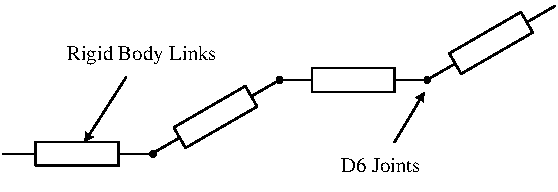
\includegraphics[width=\textwidth]{figures/cable_model_D6.pdf}
    \caption{Implementation of MSD models in the simulator.}
    \label{linkd6}
  \end{minipage}
\end{figure}

Although the mass--spring--damper (MSD) model for cable dynamics is conceptually straightforward and relatively simple to implement, numerical challenges can arise in practical simulators. In many physics engines, the internal solver for dynamics relies on iterative methods such as the Gauss--Seidel (GS) algorithm to solve systems of equations arising from joint or constraint forces. For example, consider a linear system of the form
\begin{equation}
  \mathbf{A}\,\mathbf{x} = \mathbf{b},
  \label{eq:linear_system}
\end{equation}
where \(\mathbf{A} \in \mathbb{R}^{n \times n}\) is a coefficient matrix, \(\mathbf{x} \in \mathbb{R}^n\) is the unknown vector, and \(\mathbf{b} \in \mathbb{R}^n\) is the right-hand side vector. The Gauss--Seidel method solves the equation \eqref{eq:linear_system} iteratively by updating one component of \(\mathbf{x}\) at a time, using the most recent updates as they become available:
\begin{equation}
  x_i^{(k+1)}
  = \frac{1}{a_{ii}}\Bigl(
      b_i
      - \sum_{j < i} a_{ij} \, x_j^{(k+1)}
      - \sum_{j > i} a_{ij} \, x_j^{(k)}
    \Bigr),
  \quad i = 1,2,\dots,n,
\end{equation}
where \(x_i^{(k)}\) denotes the \(i\)-th component of the vector \(\mathbf{x}\) at iteration \(k\). The iteration sweeps through \(i = 1\) to \(n\), then repeats until convergence (or failure to converge).

In an MSD system, each cable or joint often introduces large entries in the global stiffness matrix \(\mathbf{A}\), particularly when the spring constant (\(k\)) or damping coefficient (\(c\)) is high. While robust time-integration schemes and solver strategies can handle moderate stiffness, when \(k\) or \(c\) become excessively large, the matrix \(\mathbf{A}\) can become ill-conditioned or exhibit very high condition numbers. This leads to the following potential issues in a Gauss--Seidel solver:

\begin{enumerate}
  \item \textbf{Slow convergence or divergence.} If \(\mathbf{A}\) is poorly conditioned, the error reduction per iteration of Gauss--Seidel can become extremely slow. In some cases, numerical round-off or small perturbations in the matrix may cause the solver to diverge rather than converge.

  \item \textbf{Stiffness-induced instability.} In real-time physics simulations, large stiffness or damping forces can make the system ``stiff,'' requiring very small time steps for stability. An iterative solver like Gauss--Seidel may not converge within the allotted iteration budget if the local coupling is too strong.

  \item \textbf{Limited numerical accuracy.} With large entries on the diagonal (due to high stiffness/damping), errors in floating-point arithmetic can accumulate, degrading precision and further hindering the iterative solver's convergence.
\end{enumerate}

When a system is too stiff, one can employ smaller time-step sizes or add numerical damping schemes to mitigate high-frequency effects. However, all of these strategies may increase computational cost and complexity, thus demanding a careful balance between physical realism, stability, and performance in the simulation of highly stiff or heavily damped MSD cable models.

\begin{figure}[H]
  \centering
  \begin{minipage}{0.65\textwidth}
    \centering
    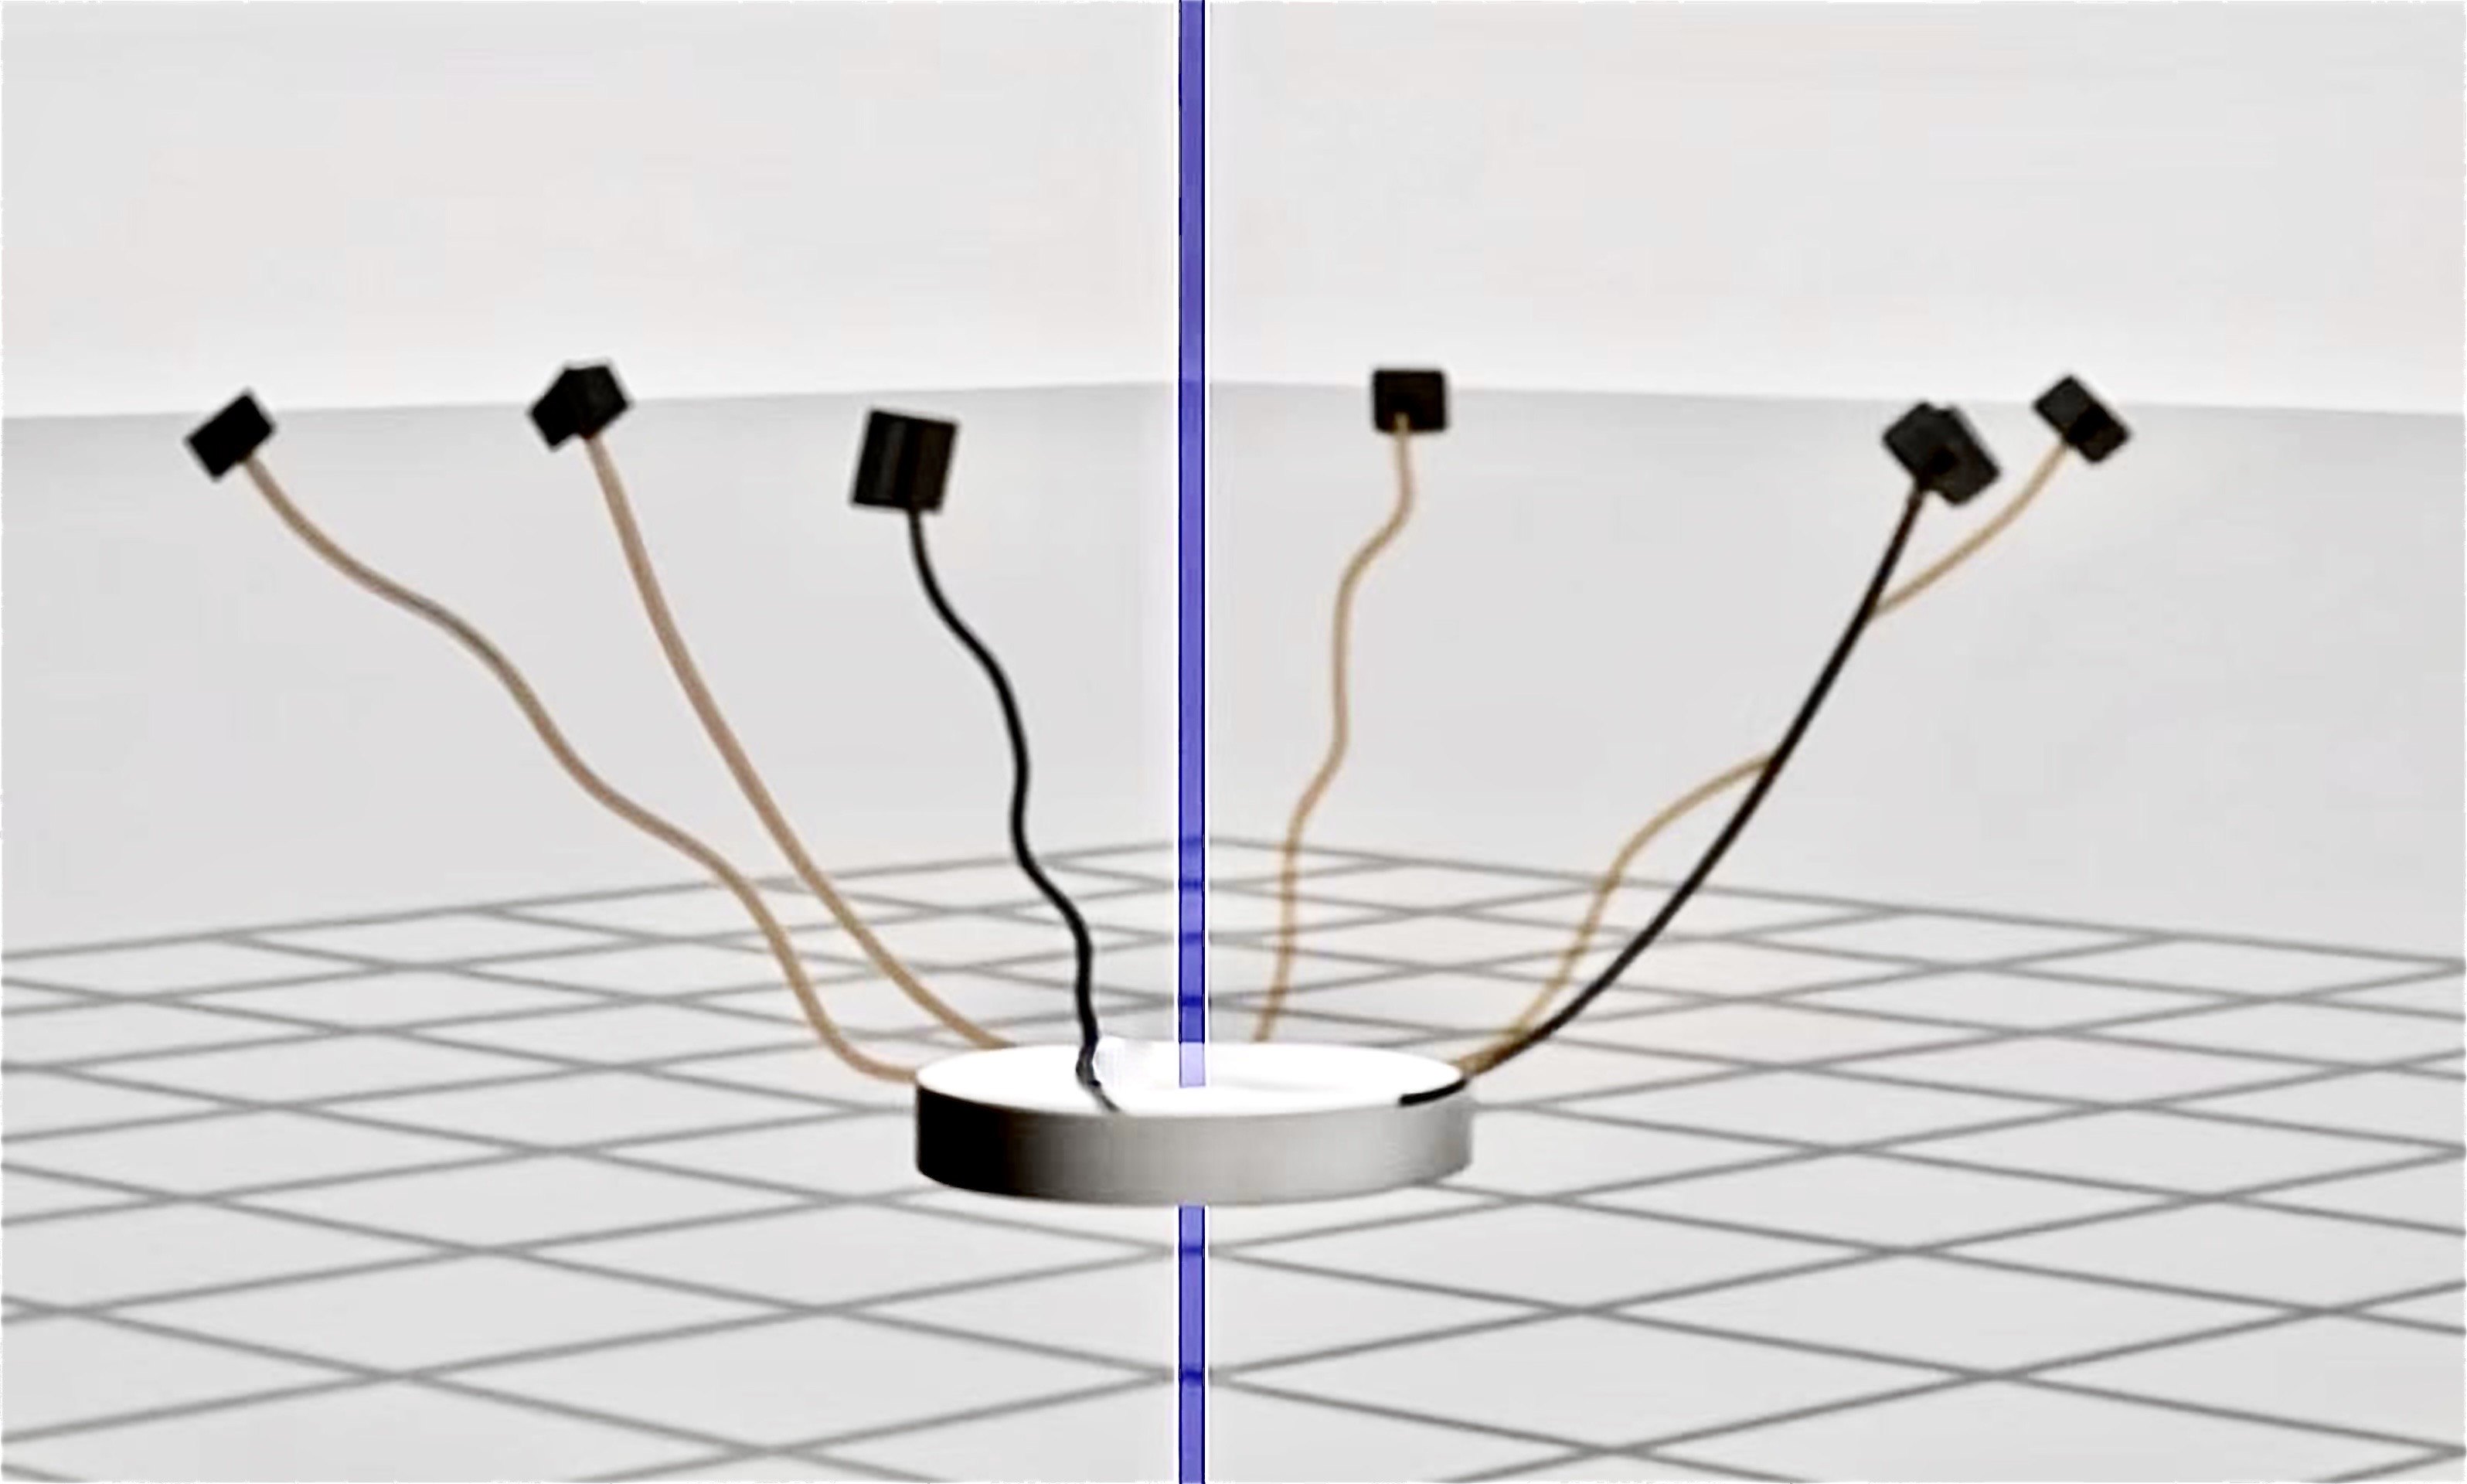
\includegraphics[width=\textwidth]{figures/fault.jpg}
    \label{failure}
  \end{minipage}
  \caption{Cable unstable oscillation resulting from Gauss-Seidel numerical failure}
\end{figure}

To address the aforementioned issues and ensure both the stability and real-time capability of the simulation, two primary strategies were adopted. First, the Temporal Gauss-Seidel (TGS) solver was employed in place of the conventional Gauss-Seidel (GS) method, offering improved numerical stability under stiff conditions. Second, soft constraints were applied to the stiffness and damping parameters, rather than enforcing them as hard constraints. The following sections provide a detailed discussion of these methods.

\paragraph{Temporal Gauss--Seidel (TGS) Solver}
Classical Gauss--Seidel (GS) and Projected Gauss--Seidel (PGS) methods often struggle with slow convergence or numerical instability in mass--spring--damper (MSD) systems characterized by high stiffness and damping. However, a \emph{Temporal Gauss--Seidel} (TGS) solver augments position-based updates with \emph{velocity-level} corrections at each iteration. This additional velocity damping better controls the rate of energy injection in the system, yielding improved stability and faster convergence for real-time applications.

In TGS, the constraint equations are formulated in velocity space. A generic velocity-based constraint has the form
\begin{equation}
  \mathbf{J}\,\mathbf{v} + \mathbf{b} = 0,
  \label{eq:tgs_constraint}
\end{equation}
where \(\mathbf{J}\) is the constraint Jacobian, \(\mathbf{v}\) is the vector of generalized velocities, and \(\mathbf{b}\) includes bias terms for Baumgarte stabilization or error reduction. At each TGS iteration, incremental impulses \(\Delta \boldsymbol{\lambda}\) are computed and used to update velocities:
\begin{equation}
  \Delta \mathbf{v} = \mathbf{M}^{-1}\,\mathbf{J}^\mathsf{T}\,\Delta \boldsymbol{\lambda},
  \label{eq:tgs_velocity_update}
\end{equation}
where \(\mathbf{M}^{-1}\) is the inverse mass-inertia matrix. The velocities and positions are then updated:
\begin{align}
  \mathbf{v}^{(k+1)} &= \mathbf{v}^{(k)} + \Delta \mathbf{v}, \\
  \mathbf{x}^{(k+1)} &= \mathbf{x}^{(k)} + \Delta t\,\mathbf{v}^{(k+1)},
  \label{eq:tgs_position_update}
\end{align}
where \(\Delta t\) is the timestep. 

Compared to standard GS or PGS, TGS explicitly handles velocity-level corrections throughout each iteration. As a result, it damps out spurious high-frequency oscillations more effectively, allowing the solver to remain stable under large stiffness or damping constants. Moreover, TGS generally requires fewer iterations to converge to a physically plausible state in real-time contexts, reducing the computational burden while preserving numerical robustness.


% \paragraph{Soft Constraints}
% In an MSD cable model, excessively large stiffness and damping parameters can introduce extreme force spikes when treated as rigid limits. Joint constraints in physics engines like NVIDIA PhysX typically include both a \emph{driver} part, which applies a proportional-derivative (PD) law to move a joint toward a target, and a \emph{limit} part, which enforces a positional boundary. PhysX's Temporal Gauss--Seidel (TGS) solver iteratively processes these constraints at each timestep to update velocities and positions such that the system as a whole converges to a physically plausible state.

% On the one hand, the drive constraint can be expressed (for a translational degree of freedom) as
% \begin{equation}
%   F_{\text{drive}} 
%   = k_{\text{drive}}\, (p_{\text{target}} - p)
%   + c_{\text{drive}}\, (v_{\text{target}} - v),
%   \label{eq:drive_force_TGS}
% \end{equation}
% where $p$ and $v$ are the current position and velocity, $p_{\text{target}}$ and $v_{\text{target}}$ are the goal position and velocity, and $k_{\text{drive}}, c_{\text{drive}}$ are stiffness and damping coefficients, respectively. On the other hand, the limit constraint remains inactive unless $p$ exceeds a boundary $p_{\max}$; once exceeded, it enforces a spring--damper response:
% \begin{equation}
%   F_{\text{limit}}
%   = -\,k_{\text{limit}} \, (p - p_{\max}) 
%     \;-\; c_{\text{limit}}\,(v),
%   \quad \text{for } p > p_{\max}.
%   \label{eq:limit_force_TGS}
% \end{equation}
% Because TGS solves constraints iteratively at each timestep, it handles the driver and limit \emph{in parallel}. If the cable segment remains within $p \le p_{\max}$, only the driver is active; if $p$ attempts to exceed $p_{\max}$, the limit constraint springs into effect to keep the segment in range.

% An excessively large drive stiffness ($k_{\text{drive}} \to 10^5$ or above) can make TGS struggle to converge when no explicit limit stiffness is in place. This happens because:
% \begin{itemize}
%   \item The solver effectively sees a ``soft infinity'' beyond $p_{\max}$; there is no explicit boundary constraint to oppose further elongation.
%   \item The drive itself must generate very high forces to counter any violation of its target, but these forces alone can lead to large velocity corrections from iteration to iteration.
%   \item Such extreme parameter values can produce ill-conditioned systems, where minor numerical errors get amplified, causing jitter or divergence.
% \end{itemize}
% By contrast, if a \emph{limit} stiffness $k_{\text{limit}}$ is configured, then once the elongation $p$ exceeds $p_{\max}$, TGS imposes a stable spring--damper force \eqref{eq:limit_force_TGS} that counteracts large deviations. This explicit boundary condition allows TGS to converge more reliably because it can ``share the load'' between the drive (which tries to reach its target) and the limit constraint (which clamps motion at $p_{\max}$). Numerical conditioning improves substantially when the solver does not rely on a single extreme stiffness to keep the system within bounds.

% Moreover, using a compliance factor $\alpha$ can soften the nominal (hard) stiffness and damping to avoid abrupt force spikes. For instance,
% \begin{equation}
%   K_{\text{limit}}^{\text{soft}}
%   = \frac{K_{\text{limit}}}{1 + \alpha_k},
%   \quad
%   C_{\text{limit}}^{\text{soft}}
%   = \frac{C_{\text{limit}}}{1 + \alpha_c},
% \end{equation}
% gradually decreases the magnitude of $k_{\text{limit}}$ and $c_{\text{limit}}$. This helps ensure that even if the drive or limit parameters must be large to capture physical behavior, they do not destabilize TGS due to excessively stiff interactions in a single iteration. Hence, combining TGS with carefully tuned drive parameters, an explicit limit constraint, and optional softening factors enables real-time MSD cable simulations with improved numerical stability, reduced oscillations, and physically consistent responses.

\paragraph{Soft Constraints}
In mass--spring--damper (MSD) cable models, imposing extremely large stiffness and damping parameters can lead to unbounded force spikes if treated as rigid constraints. In NVIDIA PhysX, each joint constraint typically comprises a \emph{driver}---which applies a proportional-derivative (PD) law to move the joint toward a target---and a \emph{limit} that enforces a positional boundary. The TGS solver iterates over these constraints at each timestep, updating velocities and positions so that the overall system converges to a physically plausible state.

Concretely, for a translational degree of freedom, the \emph{driver} constraint is modeled by
\begin{equation}
  F_{\text{drive}} 
  = k_{\text{drive}}\, \bigl(p_{\text{target}} - p\bigr)
  \;+\; c_{\text{drive}}\, \bigl(v_{\text{target}} - v\bigr),
  \label{eq:drive_force_TGS}
\end{equation}
where $p$ and $v$ are the current position and velocity, $p_{\text{target}}$ and $v_{\text{target}}$ are the desired position and velocity, and $k_{\text{drive}}$, $c_{\text{drive}}$ are the driver’s stiffness and damping coefficients. The \emph{limit} constraint remains inactive unless $p$ exceeds a boundary $p_{\max}$. When that occurs, the solver applies
\begin{equation}
  F_{\text{limit}}
  = -\,k_{\text{limit}} \, \bigl(p - p_{\max}\bigr) 
    \;-\; c_{\text{limit}}\,v,
  \quad \text{for } p > p_{\max},
  \label{eq:limit_force_TGS}
\end{equation}
to clamp motion at the boundary. During TGS iteration, these constraints are evaluated in parallel. If $p \le p_{\max}$, only the driver is active; if $p$ attempts to exceed $p_{\max}$, the limit constraint supplements the driver to keep the segment within range.

When $k_{\text{drive}}$ grows excessively large (e.g., on the order of $10^5$ or more) without a corresponding limit stiffness, TGS can struggle to converge. From the solver's perspective, any elongation beyond $p_{\max}$ must be corrected solely by very large drive forces, leading to:
\begin{itemize}
  \item No explicit boundary constraint to resist further elongation, effectively creating a ``soft infinity'' for $p>p_{\max}$.
  \item Large, rapidly changing velocities as TGS attempts to satisfy a single extreme-stiffness constraint.
  \item Ill-conditioned equations that amplify minor numerical errors, resulting in jitter or divergence.
\end{itemize}
Conversely, if a limit stiffness $k_{\text{limit}}$ is configured, then once $p$ exceeds $p_{\max}$, the solver imposes a stable spring--damper force~\eqref{eq:limit_force_TGS} rather than relying on drive forces alone. Splitting the total load between the drive (maintaining its target) and the limit constraint (clamping elongation) greatly improves numerical conditioning and convergence.

% Introducing a compliance factor $\alpha$ helps avoid abrupt force spikes by scaling down nominally large stiffness or damping. For instance,
% \begin{equation}
%   K_{\text{limit}}^{\text{soft}}
%   = \frac{K_{\text{limit}}}{1 + \alpha_{k}}, 
%   \quad
%   C_{\text{limit}}^{\text{soft}}
%   = \frac{C_{\text{limit}}}{1 + \alpha_{c}},
% \end{equation}
% lowers $k_{\text{limit}}$ and $c_{\text{limit}}$ to reduce excessive forces within a single iteration.

By combining TGS with thoughtfully chosen driver parameters and an explicit limit constraint, one can achieve real-time MSD cable simulations that offer improved numerical stability, reduced oscillations, and physically consistent behavior.


\newpage


\section{Multilift Algorithm Implementation}
\subsection{Low-level Controller}
A geometric controller\cite{geose3} operates directly on the configuration space \(\mathrm{SO}(3)\) to ensure robust and globally valid rotational error definitions. In the context of multirotor platforms, the position dynamics can be separated from the attitude dynamics by using geometric principles, while the yaw angle is decoupled to allow independent heading control\cite{geoyaw}. This approach makes it possible to design a low-level controller that regulates both the thrust (for position tracking) and the body orientation (for attitude tracking) in a coherent framework.

Consider a multirotor with position \(\mathbf{x} \in \mathbb{R}^3\) and orientation \(R \in \mathrm{SO}(3)\). Let \(\mathbf{x}_d\) be the desired position trajectory, and \(\dot{\mathbf{x}}_d\), \(\ddot{\mathbf{x}}_d\) be the desired velocity and acceleration. Let \(\psi_d\) be the desired yaw angle. We define the position and velocity errors as
\begin{equation}
\mathbf{e}_p = \mathbf{x} - \mathbf{x}_d, 
\quad
\mathbf{e}_v = \dot{\mathbf{x}} - \dot{\mathbf{x}}_d.
\end{equation}
A simple proportional-derivative-based desired acceleration command for position tracking can be formulated as
\begin{equation}
\mathbf{a}_d = \ddot{\mathbf{x}}_d 
- k_p\,\mathbf{e}_p 
- k_v\,\mathbf{e}_v 
+ g \mathbf{e}_3,
\end{equation}
where \(\mathbf{e}_3 = [0 \;\; 0 \;\; 1]^\top\) represents the global vertical axis, \(g\) is the gravitational acceleration, and \(k_p, k_v > 0\) are proportional and derivative gains.

The total thrust command \(f\) is then given by
\begin{equation}
f = m \|\mathbf{a}_d\|,
\end{equation}
where \(m\) is the mass of the vehicle. To find the desired orientation \(R_d\) that orients the body \(z\)-axis toward \(\mathbf{a}_d\) while simultaneously achieving the desired yaw \(\psi_d\), we define
\begin{equation}
\hat{\mathbf{b}}_3 = \frac{\mathbf{a}_d}{\|\mathbf{a}_d\|}, 
\end{equation}
which is the desired body \(z\)-axis direction. The desired body \(x\)-axis \(\hat{\mathbf{b}}_1\) is chosen to lie in the horizontal plane according to the desired yaw angle \(\psi_d\). One way to obtain \(\hat{\mathbf{b}}_1\) is
\begin{equation}
\hat{\mathbf{b}}_{1}^{*} = 
\begin{bmatrix}
\cos(\psi_{d}) \\
\sin(\psi_{d}) \\
0
\end{bmatrix},
\quad
\hat{\mathbf{b}}_{2} = \frac{\hat{\mathbf{b}}_{3} \times \hat{\mathbf{b}}_{1}^{*}}{\|\hat{\mathbf{b}}_{3} \times \hat{\mathbf{b}}_{1}^{*}\|},
\quad
\hat{\mathbf{b}}_{1} = \hat{\mathbf{b}}_{2} \times \hat{\mathbf{b}}_{3}.
\end{equation}

\begin{equation}
R_{d} = 
\begin{bmatrix}
\hat{\mathbf{b}}_{1} & \hat{\mathbf{b}}_{2} & \hat{\mathbf{b}}_{3}
\end{bmatrix}.
\end{equation}
This construction enforces the decoupling of yaw, because \(\psi_d\) is used explicitly to shape the desired heading, while the other two axes are defined by the thrust direction.

Attitude errors can be defined in a global, coordinate-free way using the fact that if \(R_d \in \mathrm{SO}(3)\) is the desired orientation, then the orientation error \(e_R\) and angular velocity error \(e_\Omega\) can be set as
\begin{equation}
e_R = \frac{1}{2} \bigl(R_d^T R - R^T R_d \bigr)^\vee, 
\quad
e_\Omega = \Omega - R^T R_d\,\Omega_d,
\end{equation}
where \(\Omega\) is the body angular velocity, \(\Omega_d\) is the desired angular velocity derived from the reference, and \((\cdot)^\vee\) maps a skew-symmetric matrix in \(\mathfrak{so}(3)\) to \(\mathbb{R}^3\). A typical feedback control law for the moment \(\mathbf{M}\) is
\begin{equation}
\mathbf{M} 
= -k_R\,e_R 
- k_\Omega\,e_\Omega 
+ \Omega \times J\,\Omega 
- J \bigl(\hat{\Omega} R^T R_d \Omega_d - R^T R_d\,\dot{\Omega}_d \bigr),
\end{equation}
where \(k_R, k_\Omega > 0\) are gains, \(J\) is the inertia matrix, and \(\hat{\Omega}\) is the skew-symmetric matrix representation of \(\Omega\). This ensures that the actual orientation \(R\) follows \(R_d\) while allowing for an independent yaw specification.

In summary, the geometric controller with decoupled yaw control provides a unified way to track position and yaw independently by constructing the desired orientation matrix from the desired thrust direction and yaw angle. This approach leverages \(\mathrm{SO}(3)\)-based error definitions to avoid singularities and discontinuities, yielding a smooth and globally valid low-level controller.

\subsection{SITL System Design}
\label{sec:sitl_system_design}

Figure~\ref{fig:sys_implement} depicts the software-in-the-loop (SITL) architecture that integrates the PX4 autopilot, Isaac Sim, ROS~2, and the Auto-Multilift algorithm into a cohesive simulation environment. Communication interface is established between the PX4 firmware and Isaac Sim through MAVLink, ensuring that simulated sensor data and flight commands are exchanged accurately in real time. The simulator provides high-fidelity sensor outputs, while PX4 responds with motor commands for attitude and position control.

On the ROS~2 side, several specialized nodes handle trajectory planning, high-level control, and data synchronization. The Geometric Control node processes state estimates from PX4 and generates reference attitudes and thrust commands to maintain stable flight. These references incorporate decoupled yaw regulation, thereby allowing the heading to be controlled independently of thrust and pitch–roll dynamics. Meanwhile, a separate Trajectory Planner node computes mission waypoints for multi-lift operations from the MPC Planner, where the Auto-Multilift method adjusted key parameters of MPC to improve tracking performance and robustness.

This SITL pipeline employs an additional time-synchronization mechanism to minimize latency and drift across multiple UAVs and ROS~2. A specialized node broadcasts clock updates, aligning measurement and control signals to a consistent temporal reference. Meanwhile, PX4 and Isaac Sim remain synchronized through a built-in lockstep procedure. By combining accurate multi-UAV load-transport simulations with flight-proven control software, the SITL setup provides a robust platform for validating the proposed methods before transitioning to physical flight tests.

\begin{figure}
    \centering
    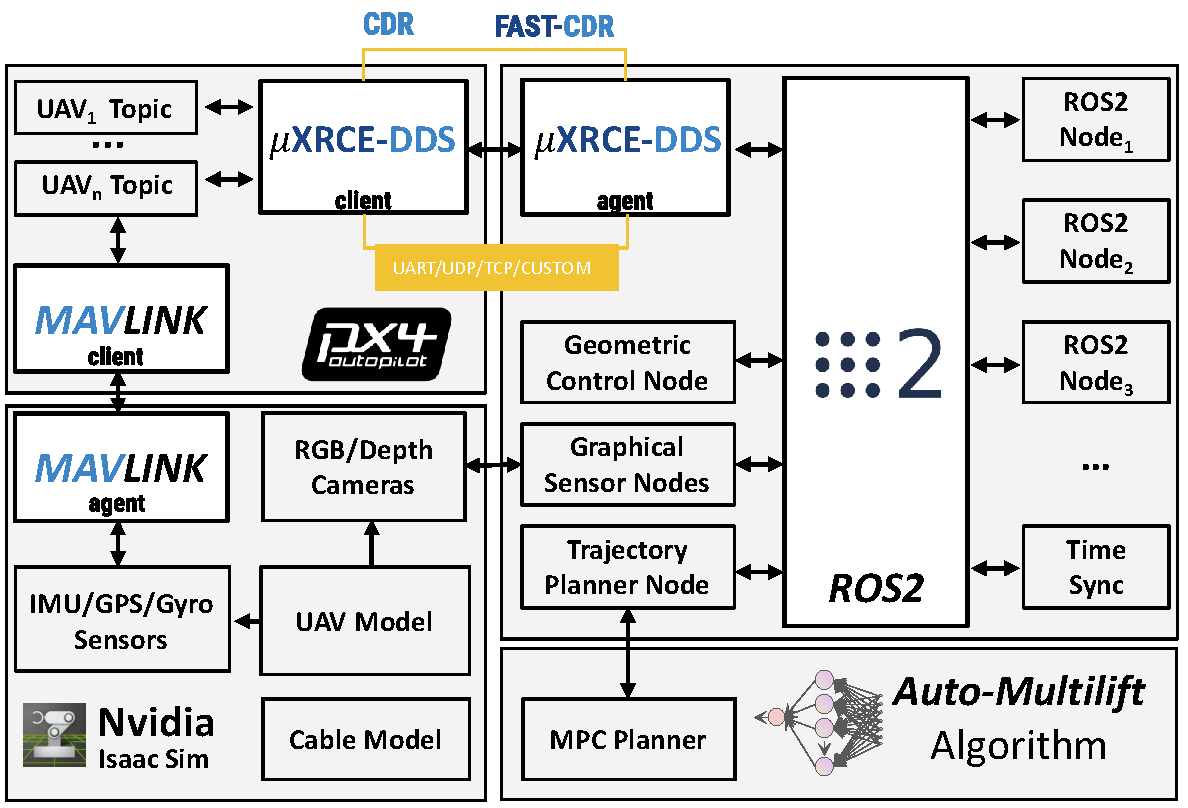
\includegraphics[width=\linewidth]{figures/sys3.pdf}
    \caption{SITL framework for Auto-Multilift}
    \label{fig:sys_implement}
\end{figure}


\newpage
\section{Experiments \& Results}
\subsection{Cable Dynamics Test}
To verify that our cable simulation behaves as intended, we conducted a series of experiments in which the overall cable stiffness and damping were set to \(10^5\)\,N/m and \(10^3\)\,Ns/m, respectively.
The primary goal of these experiments was to assess the accuracy of the cable’s elasticity modeling and the real-time performance of the simulation.
Throughout the experiments, the theoretical model of cables was considered as an ideal second-order system characterized by a stiffness of \(10^5\)\,N/m and a damping coefficient of \(10^3\)\,Ns/m along its extension.
This theoretical model forms the basis for evaluating the cable’s elongation accuracy.

We designed two main experiments. In the first experiment, weights ranging from 0.1\,kg to 5\,kg were suspended from a single rope and allowed to fall freely under gravity.
Displacements, determined by the interplay of gravitational and tensile forces, were then measured.
In the second experiment, a multi-rope configuration was employed, in which six ropes were arranged at angles 30\(^\circ\)  from the vertical.
The displacement curves for the suspended weights were recorded and compared against theoretical predictions.

\begin{figure}[ht]
    \centering
    \begin{minipage}[t]{0.49\linewidth}
        \centering
        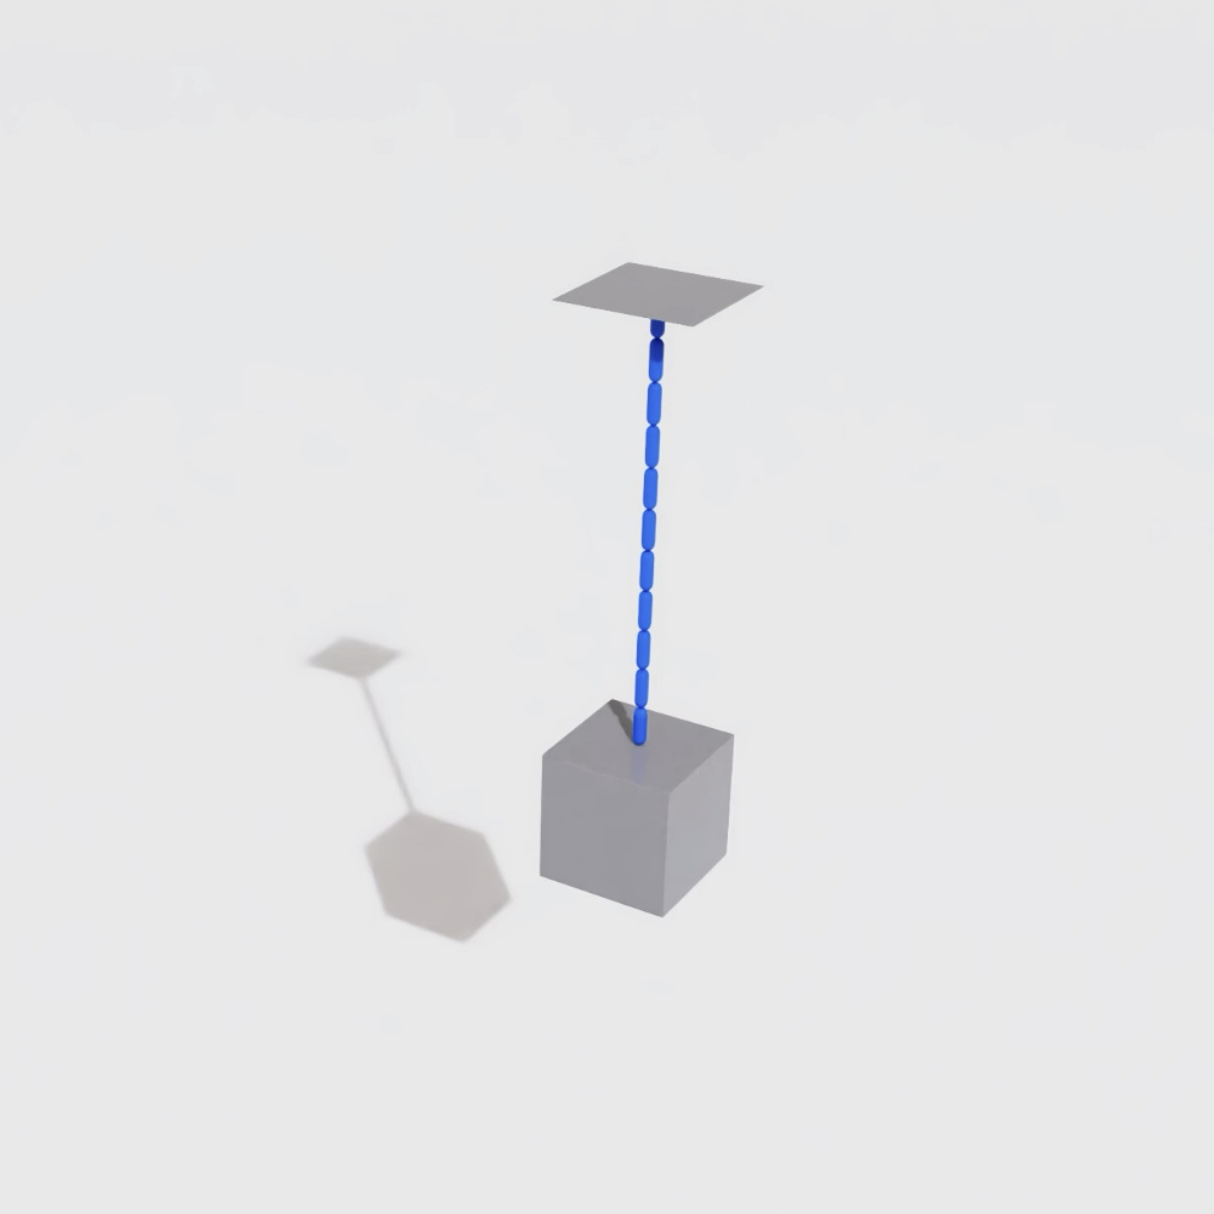
\includegraphics[width=\linewidth]{figures/single_test.jpg}
        \caption{Single cable test scene}
        \label{fig:single_test}
    \end{minipage}
    \hfill
    \begin{minipage}[t]{0.49\linewidth}
        \centering
        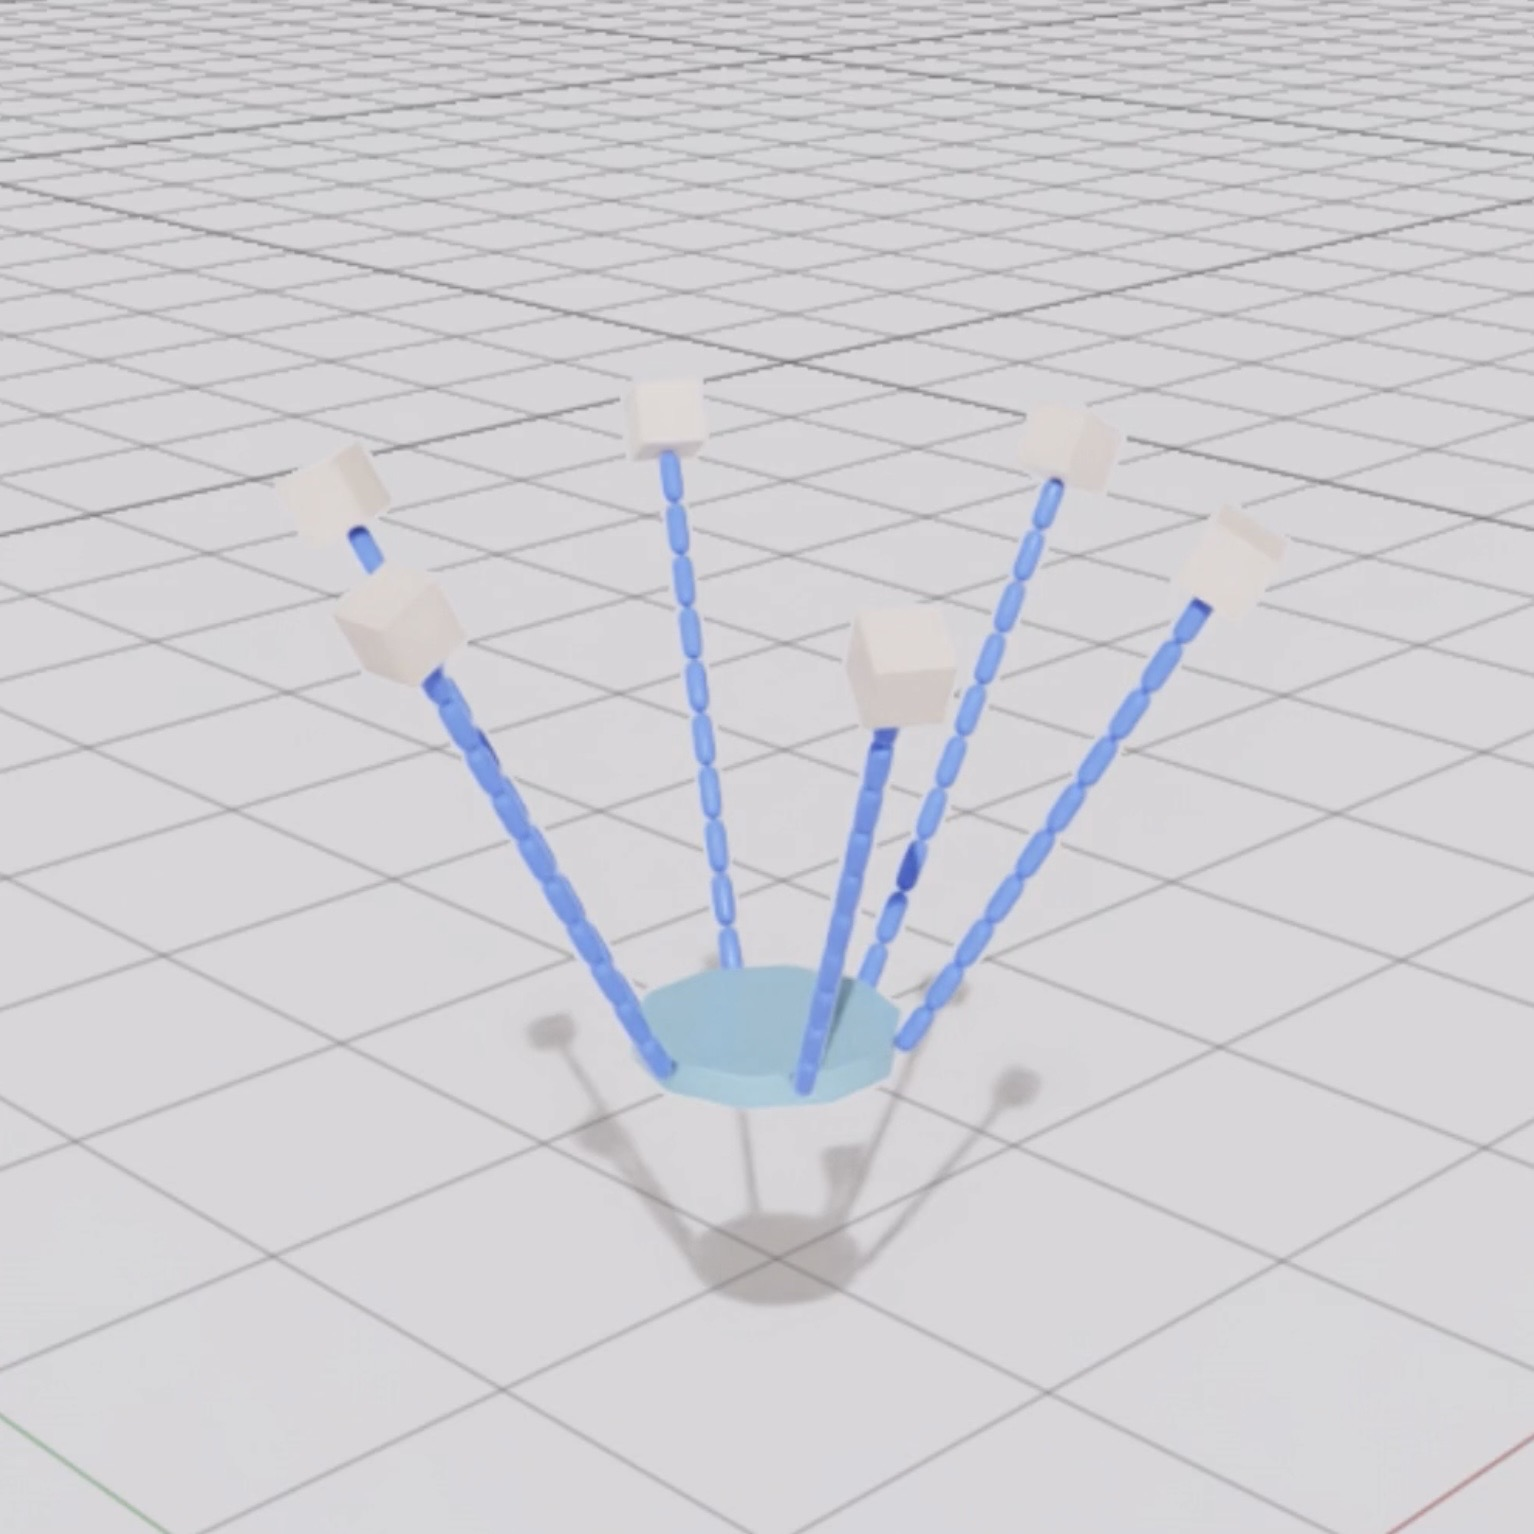
\includegraphics[width=\linewidth]{figures/multi_test.jpg}
        \caption{Six cable test scene}
        \label{fig:multi_test}
    \end{minipage}
\end{figure}

Table~\ref{tab:single_cable_results} summarizes the representative single-cable results. The tested stiffness values remain close to \(10^5\,\text{N/m}\), with a maximum relative error of 2.2\%. These data confirm that the simulation captures the cable’s elasticity well, especially given the wide range of payloads tested. This also indicates that during the process of numerical iteration of the simulation, the damping force determined by the chosen damping coefficient, \(10^3\,\text{Ns/m}\), provides a sufficiently rapid settling time without causing a numerical instability.

\begin{table}[ht]
    \centering
    \caption{Results of the single-cable test for varying payload masses.}
    \label{tab:single_cable_results}
    \begin{tabular}{ccc}
    \toprule
    \makebox[0.25\textwidth][c]{\textbf{Payload (kg)}} & 
    \makebox[0.35\textwidth][c]{\textbf{Tested Stiffness (N/m)}} & 
    \makebox[0.30\textwidth][c]{\textbf{Relative Error (\%)}} \\
    \midrule
    0.1 & $1.000\times10^5$ & 0.0 \\
    0.5 & $1.000\times 10 ^5$ & 0.0 \\
    1.0 & $9.995\times10^4$ &  0.5\\
    5.0 & $9.978\times10^4$ & 2.2 \\
    \bottomrule
    \end{tabular}
\end{table}

Figures~\ref{fig:case1}--\ref{fig:case4} illustrate how the elongations of single cables evolve under various mass of payloads. In each case, the rope elongation exhibits small oscillations around the expected theoretical second-order response, settling rapidly toward the predicted equilibrium.
 These minor deviations stem from numerical rounding in the real-time simulation but remain within acceptable margins. Overall, the tests validate that our model’s stiffness and damping parameters yield physically consistent dynamics and maintain stability across different load conditions.


\begin{figure}[H]
    \centering
    \begin{minipage}{0.49\textwidth}
        \centering
        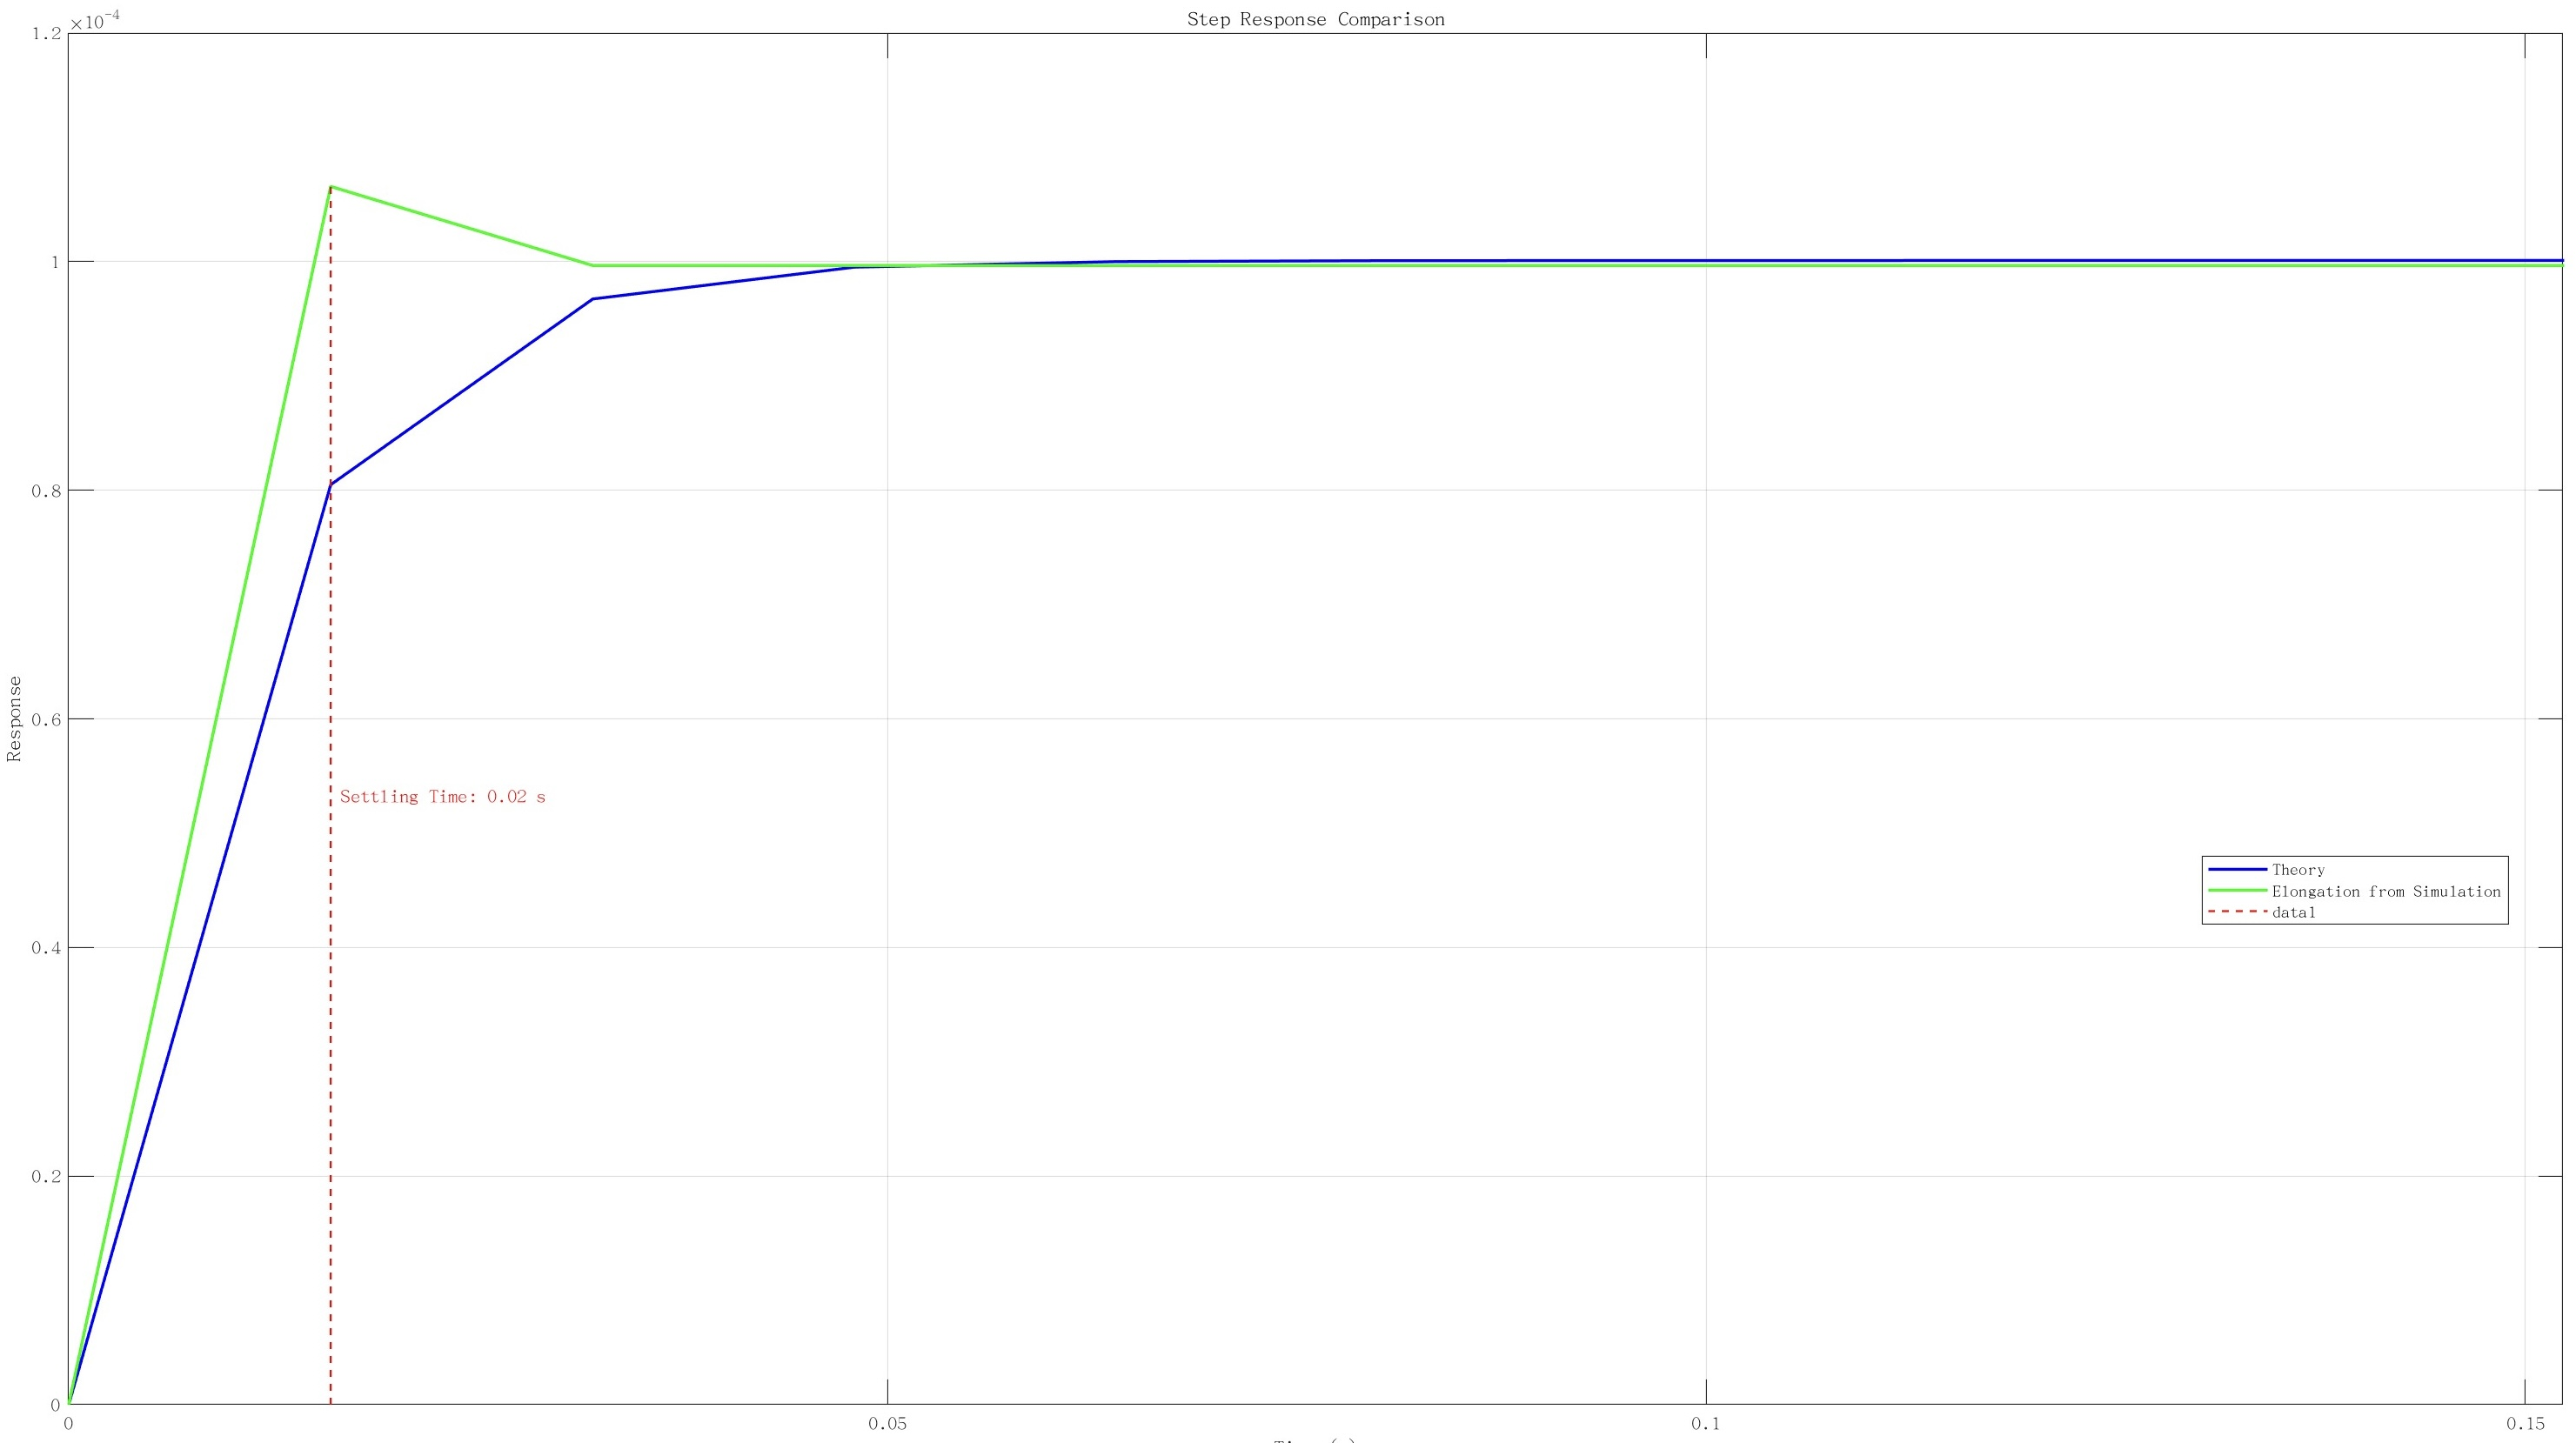
\includegraphics[width=\linewidth]{figures/0.1s.jpg}
        \caption{Single cable with 0.1 Kg payload}
        \label{fig:case1}
    \end{minipage}
    \hfill
    \begin{minipage}{0.49\textwidth}
        \centering
        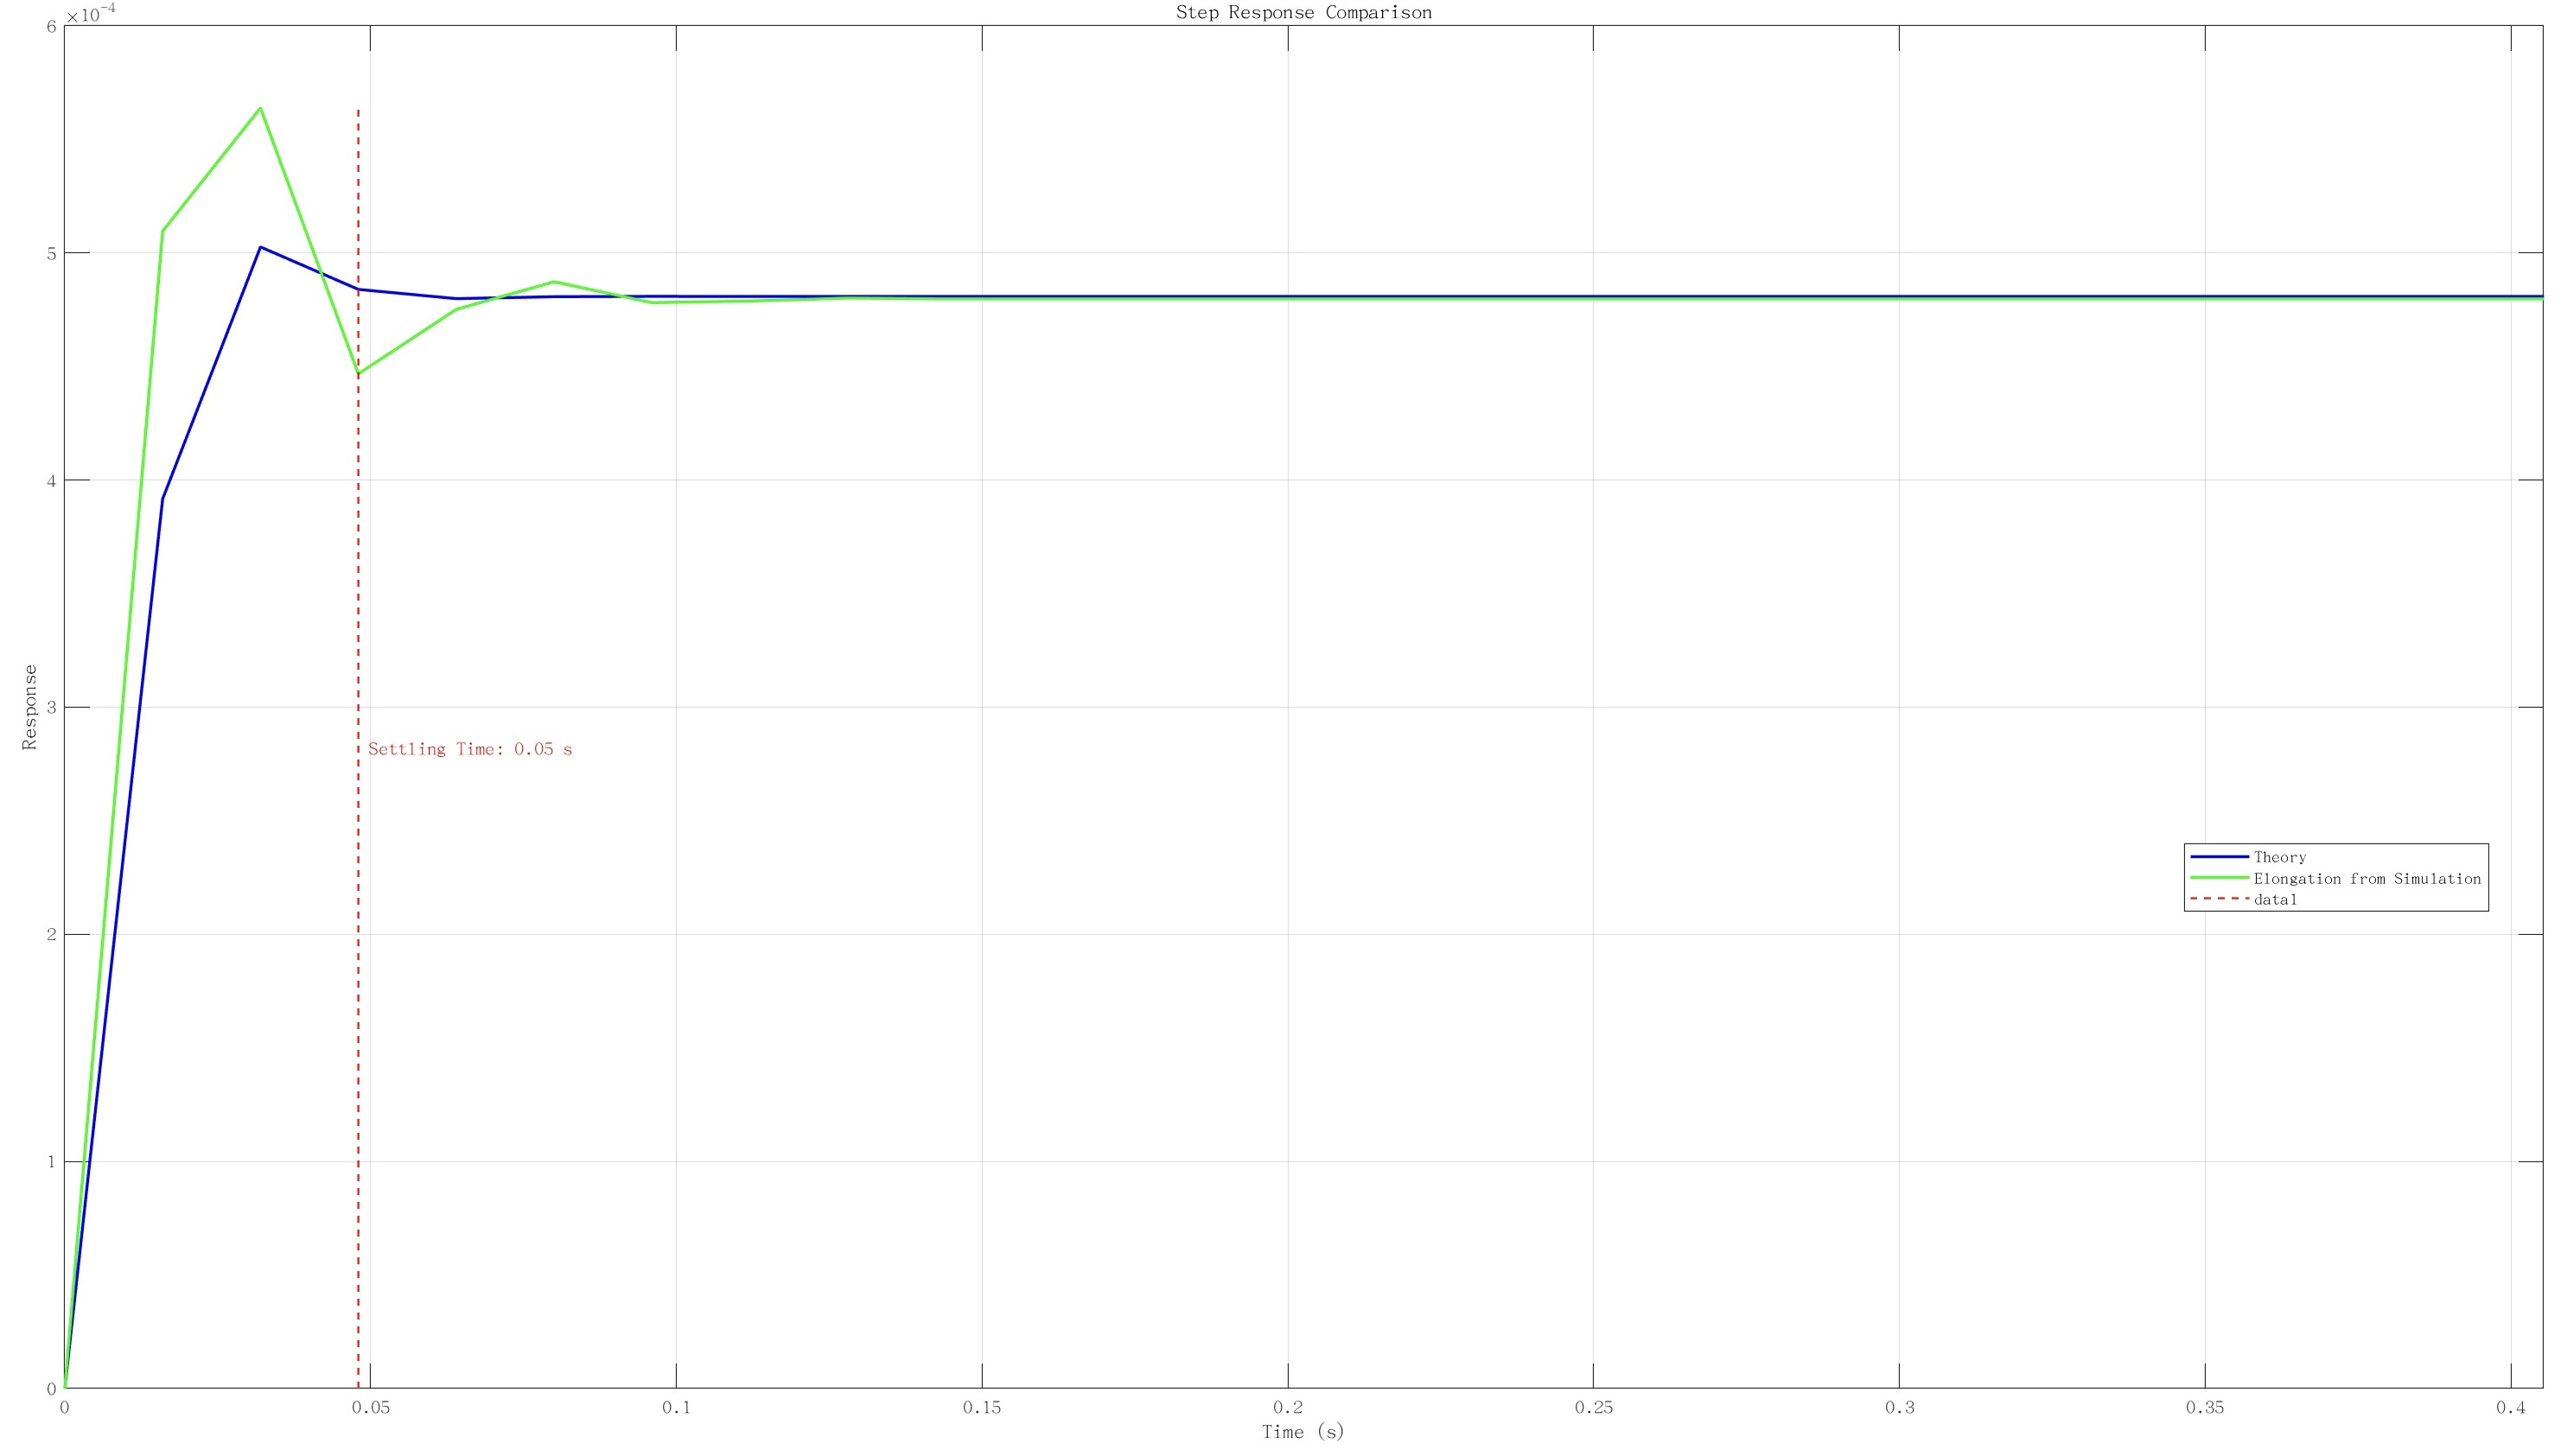
\includegraphics[width=\linewidth]{figures/0.5s.jpg}
        \caption{Single cable with 0.5 Kg payload}
        \label{fig:case2}
    \end{minipage}
    
    \vspace{0.5cm}

    \begin{minipage}{0.49\textwidth}
        \centering
        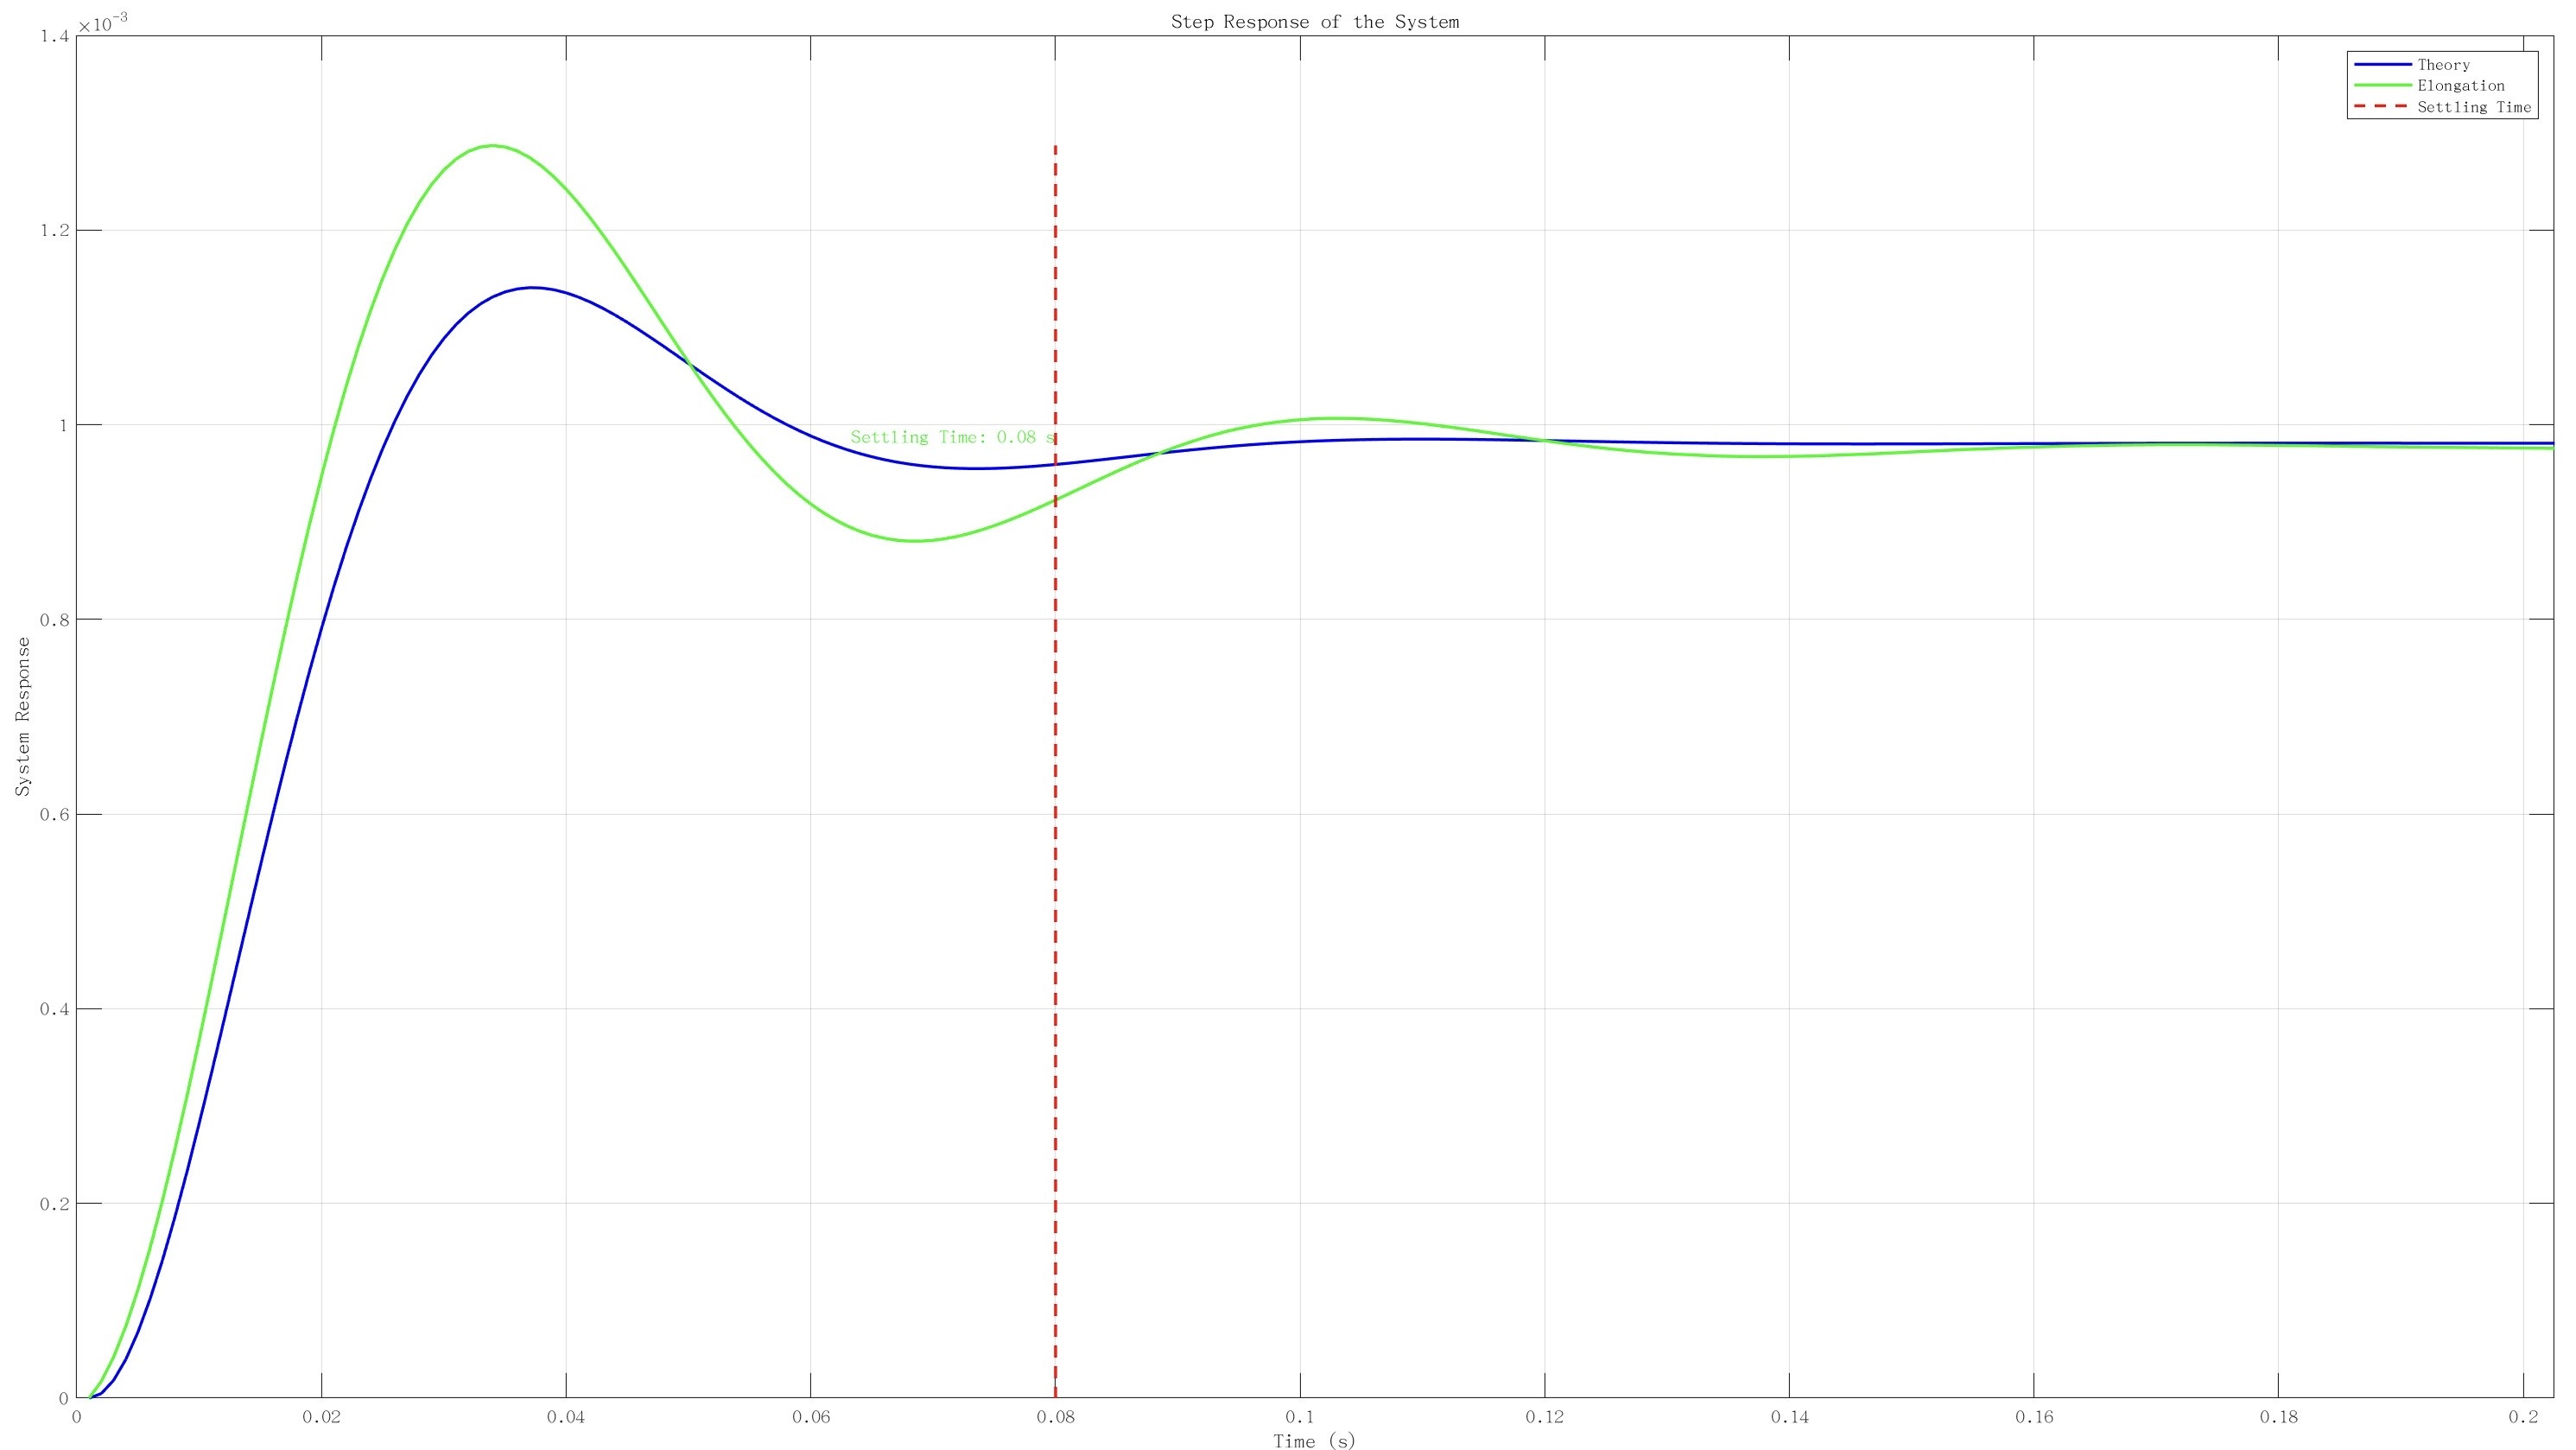
\includegraphics[width=\linewidth]{figures/1s.jpg}
        \caption{Single cable with 1 Kg payload}
        \label{fig:case3}
    \end{minipage}
    \hfill
    \begin{minipage}{0.49\textwidth}
        \centering
        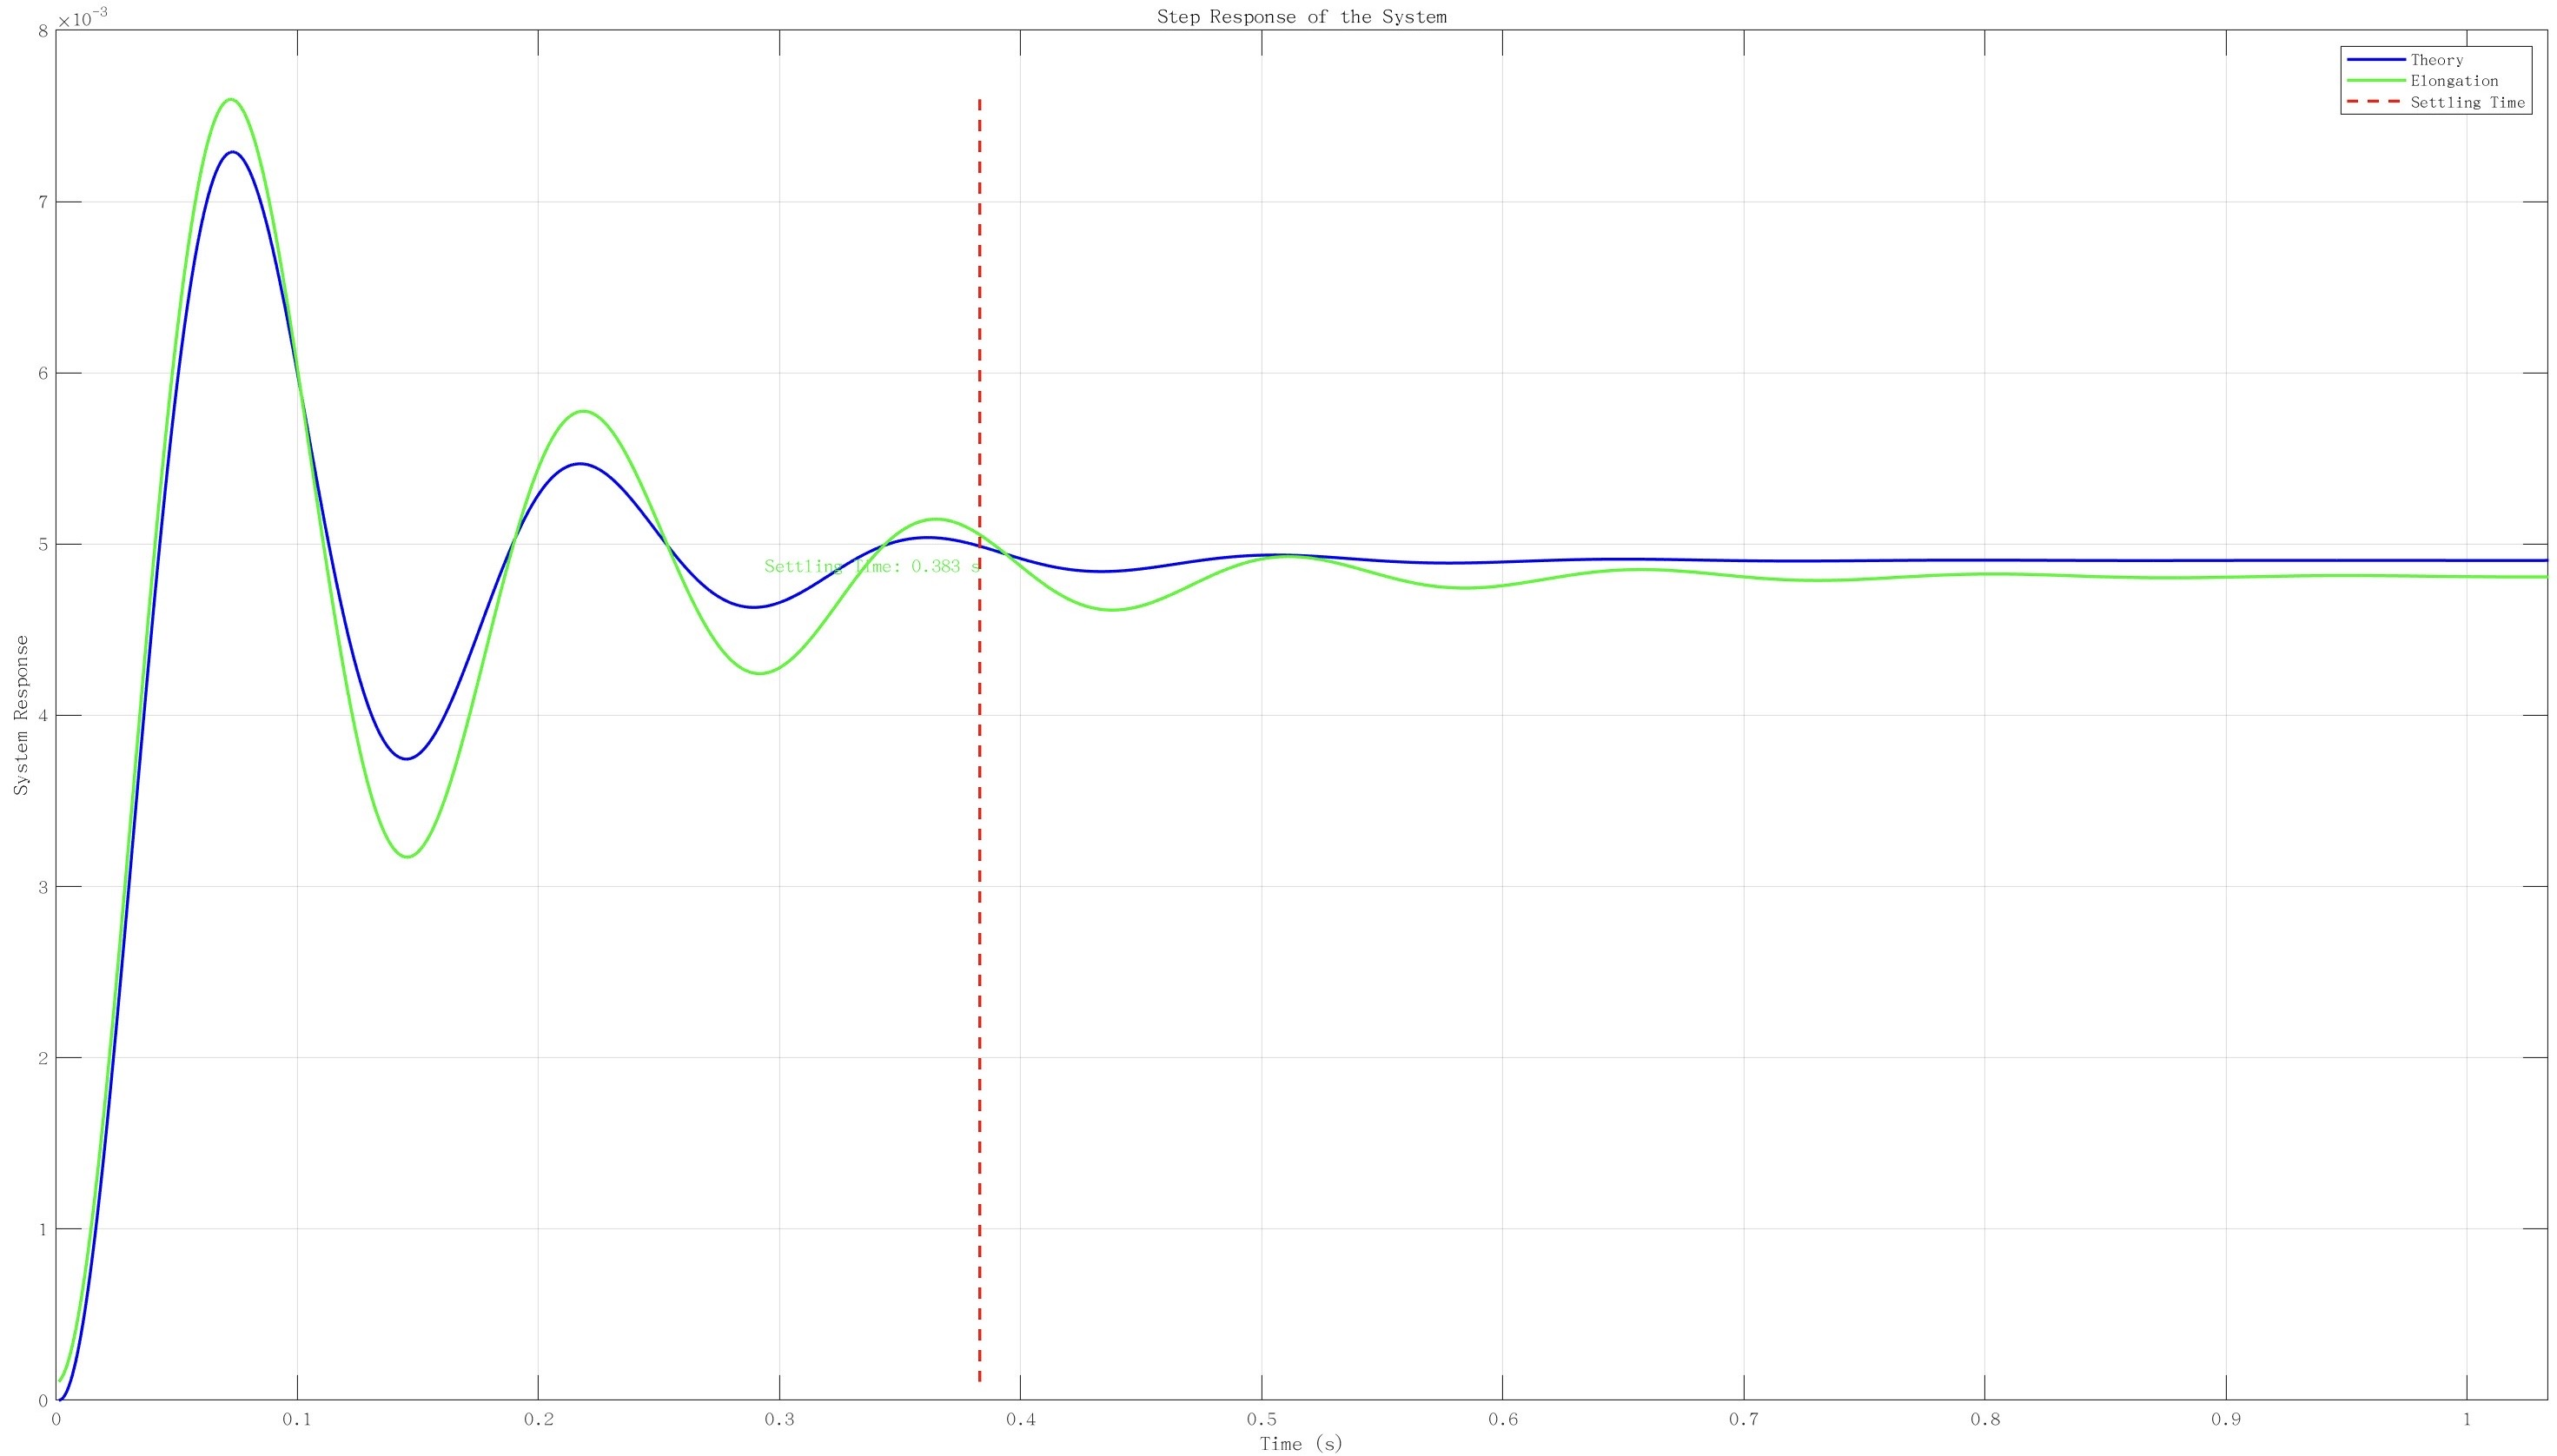
\includegraphics[width=\linewidth]{figures/5s.jpg}
        \caption{Single cable with 5 Kg payload}
        \label{fig:case4}
    \end{minipage}
\end{figure}


Figure~\ref{fig:multi1}-\ref{fig:multi3} present the results of the six-cable experiments conducted with varying payload masses.
\begin{figure}[H]
    \centering
    \begin{minipage}{0.32\textwidth}
        \centering
        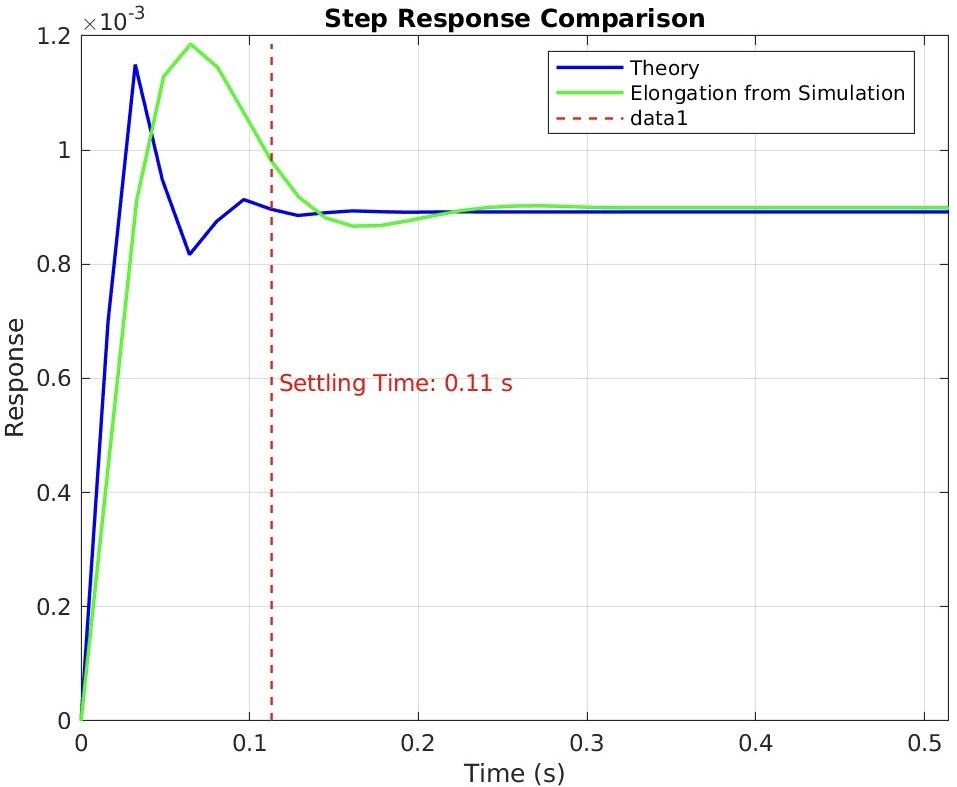
\includegraphics[width=\linewidth]{figures/multi_6.jpg}
        \caption{6 cables with 6 Kg payload}
        \label{fig:multi1}
    \end{minipage}
    \hfill
    \begin{minipage}{0.32\textwidth}
        \centering
        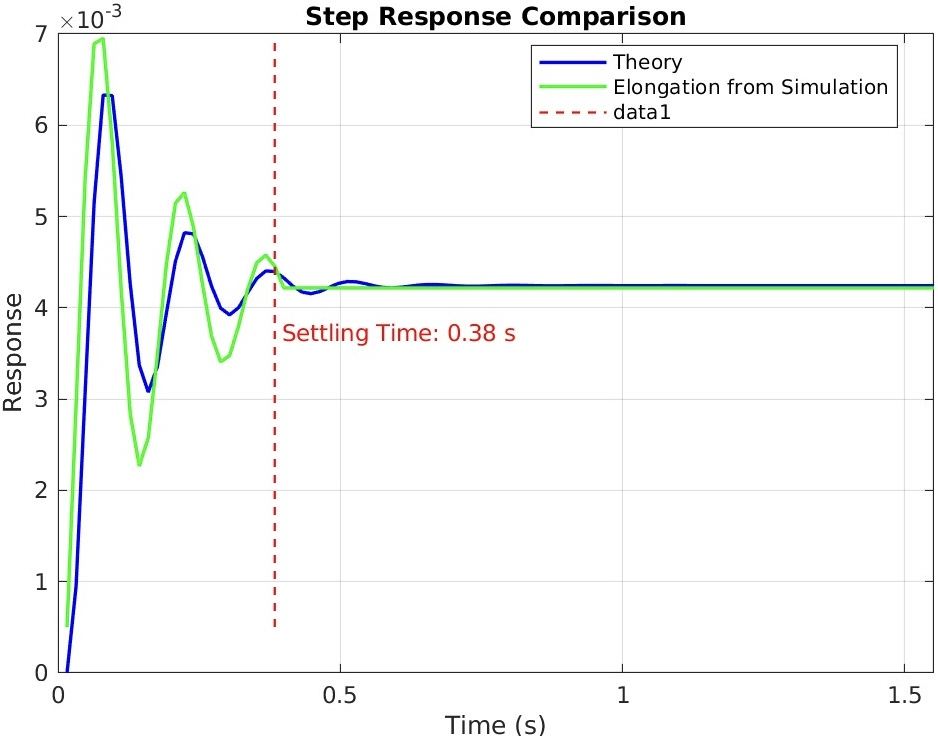
\includegraphics[width=\linewidth]{figures/multi_30.jpg}
        \caption{6 cables with 30 Kg payload}
        \label{fig:multi2}
    \end{minipage}
    \hfill
    \begin{minipage}{0.32\textwidth}
        \centering
        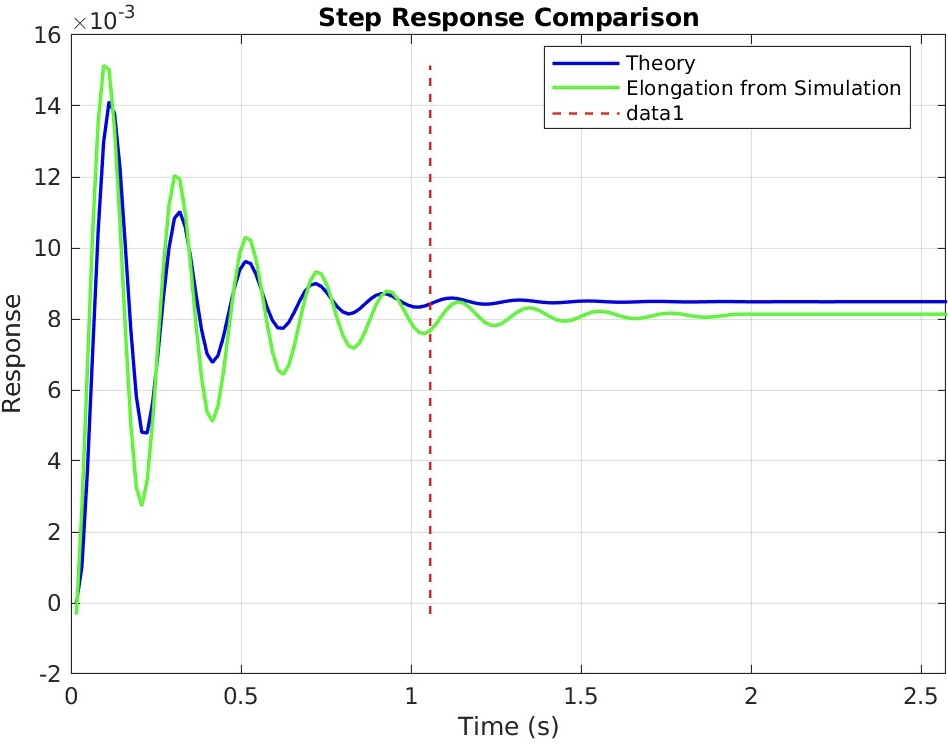
\includegraphics[width=\linewidth]{figures/multi_60.jpg}
        \caption{6 cables with 60 Kg payload}
        \label{fig:multi3}
    \end{minipage}
\end{figure}

As illustrated in Figures~\ref{fig:multi1}--\ref{fig:multi3}, the multi-cable system can be simulated in real time while maintaining excellent agreement with theoretical predictions across a wide range of payload masses. For lighter payloads (e.g., 6\,kg), the system displays mild overshoot and rapid settling, consistent with classic second-order system behavior. Increasing the payload to 30\,kg and 60\,kg introduces more noticeable oscillations and longer settling times, which match the anticipated decrease in natural frequency for higher mass-to-stiffness ratios. 

Despite these larger oscillations at higher loads, the simulated elongation remains centered around the theoretical curve, indicating both numerical stability and high physical accuracy. These findings confirm that the multi-cable system—designed with the specified stiffness and damping parameters—delivers real-time performance without compromising on fidelity, accurately capturing force distribution and dynamic effects even in challenging multi-rope scenarios.

\subsection{Multilift Trajectory Following}
To comprehensively assess the design of the SITL multi-lift system, we conducted a detailed trajectory-following experiment in which each quadrotor was commanded to travel along a horizontal circular path with a 5,m radius, at a constant angular velocity of 0.2,rad/s. The linear velocity for each quadrotor is therefore 2,m/s. This circular motion ensures that the system experiences continuous, varying orientations of tension and load distribution among the drones. Additionally, each drone’s yaw angle was continuously adjusted so that its forward axis aligned tangentially to the circle, keeping the drone oriented in the direction of travel. By enforcing these conditions, the experiment provides a rigorous test of the geometric controller’s ability to maintain both formation and accurate tracking. The experiment offers valuable insight into the overall system stability under dynamic load-sharing and highlights how effectively the geometric controller can execute coordinated maneuvers in real time.

The different states of the quadrotors during this experiment—takeoff, hover, and task execution—are shown in Figure~\ref{fig:takeoff}-\ref{fig:task}. As illustrated in these figures, the system transitions smoothly from a static ground state into a fully airborne formation without significant overshoot or drift. During the \emph{takeoff} phase (Figure~\ref{fig:takeoff}), the quadrotors ascend while maintaining relative positions; cables remain slack and show its flexibility.  In the \emph{hover} phase (Figure~\ref{fig:hover}), each vehicle maintains a stable altitude above the ground, allowing us to verify that the geometric controller can hold the formation in place with minimal oscillation. Finally, in the \emph{task} phase (Figure~\ref{fig:task}), the quadrotors proceed along the circular path with precise velocity and orientation control, thus achieving the trajectory-following objective.

\begin{figure}[H]
    \centering
    \begin{minipage}{0.32\textwidth}
        \centering
        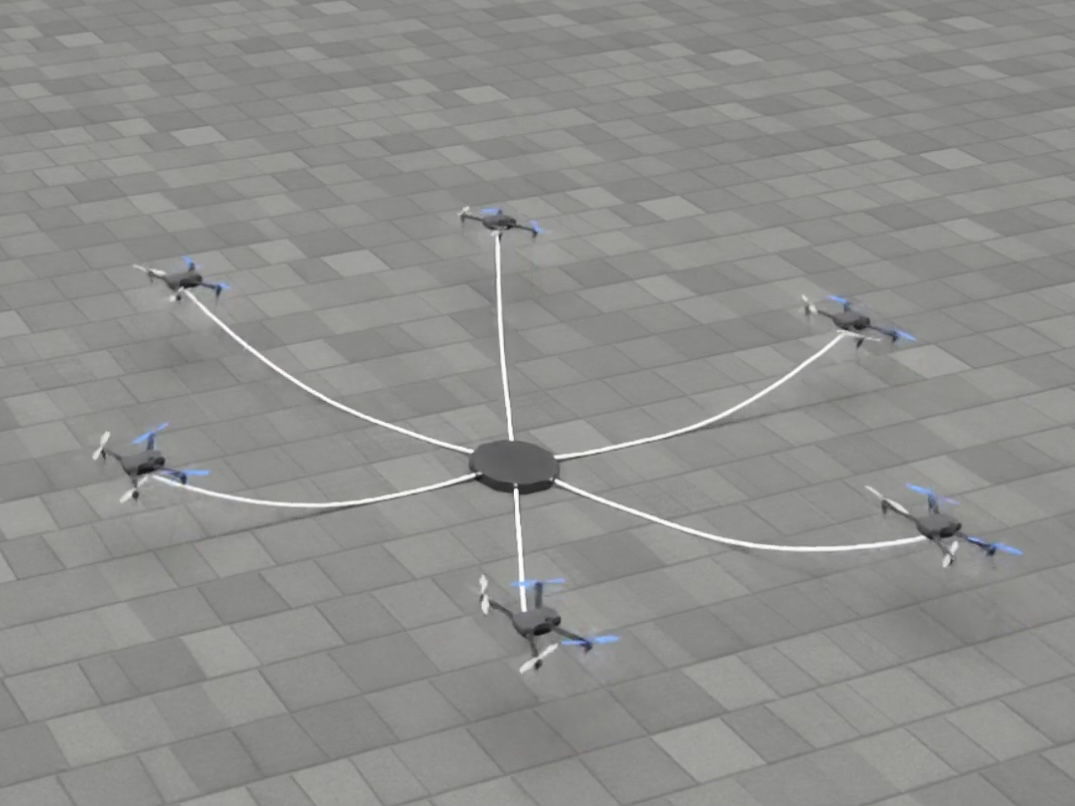
\includegraphics[width=\linewidth]{figures/takeoff.jpg}
        \caption{Takeoff}
        \label{fig:takeoff}
    \end{minipage}
    \hfill
    \begin{minipage}{0.32\textwidth}
        \centering
        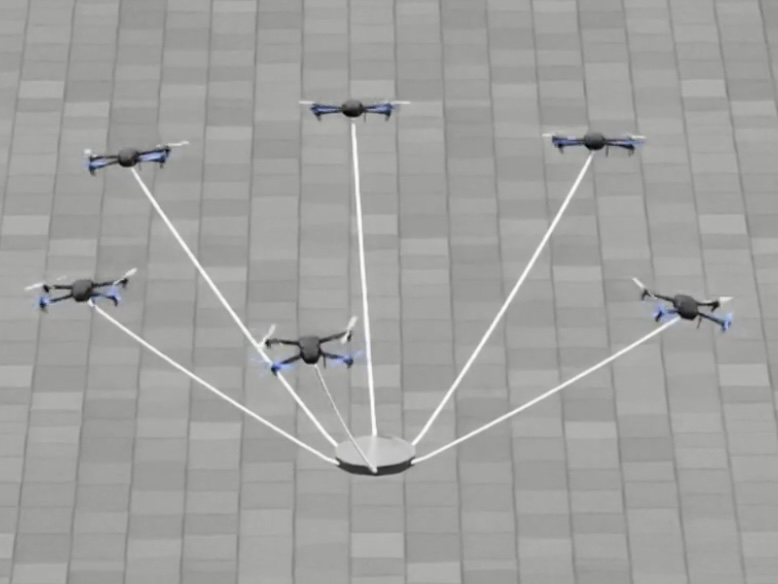
\includegraphics[width=\linewidth]{figures/hover.jpg}
        \caption{Hover}
        \label{fig:hover}
    \end{minipage}
    \hfill
    \begin{minipage}{0.32\textwidth}
        \centering
        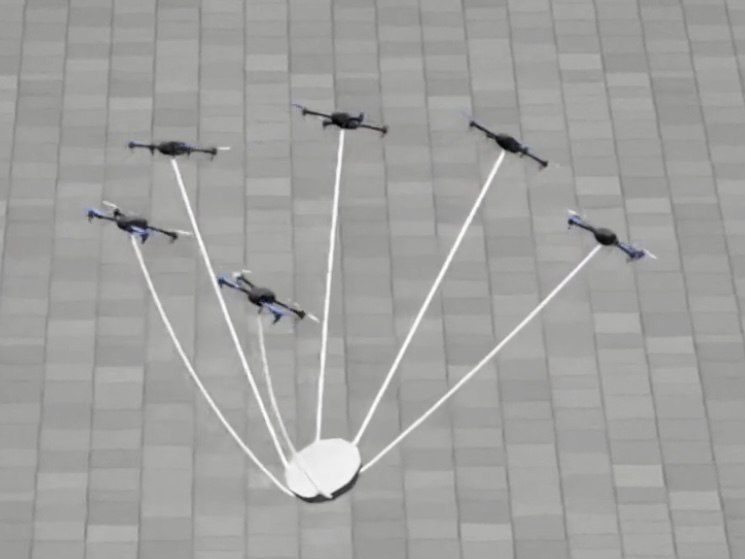
\includegraphics[width=\linewidth]{figures/spin.jpg}
        \caption{Task}
        \label{fig:task}
    \end{minipage}
\end{figure}

The position and orientation tracking errors for individual quadrotors were also monitored throughout the experiment. The trajectory for one of the drones is visualized in Figure \ref{fig:track}. Average position-tracking errors remained under 3\,cm from the reference trajectory, underscoring the effectiveness of the control algorithm in regulating the system’s translational dynamics. Meanwhile, the yaw angles consistently followed the intended tangential orientation, with deviations not exceeding 1\(^\circ\). These results demonstrate the capacity of the multi-lift system to maintain coherent, formation-level control, even under relatively high-speed maneuvers.

\begin{figure}[H]
    \centering
    \begin{minipage}{\textwidth}
        \centering
        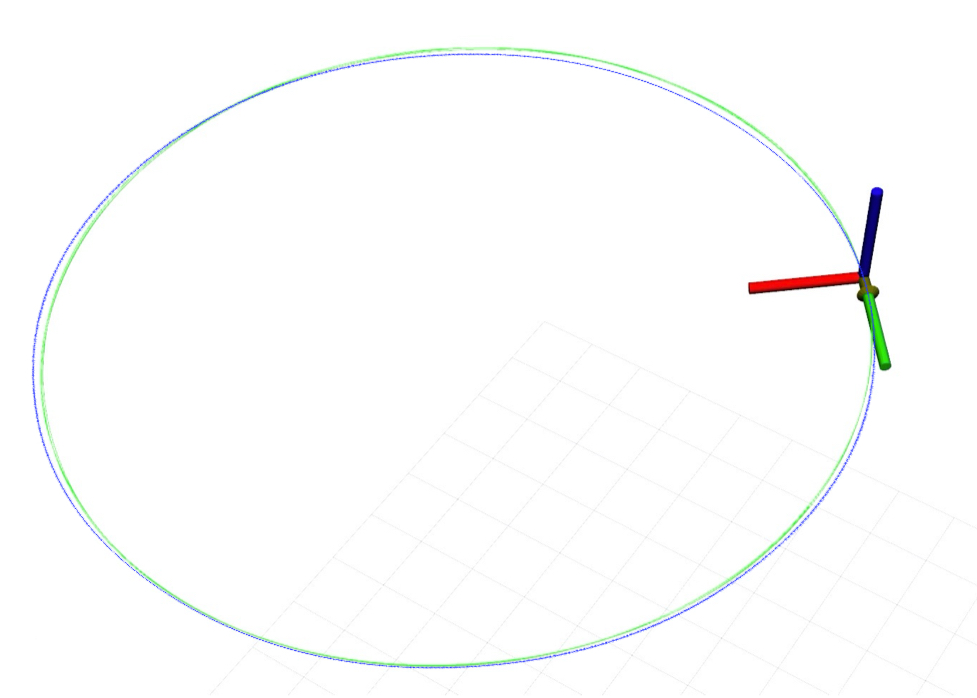
\includegraphics[width=0.45\linewidth]{figures/track.jpg}
        \caption{Trajectory tracking visualization in Rviz}
        \label{fig:track}
    \end{minipage}
\end{figure}

Overall, the multilift trajectory-following experiment validates the system’s ability to coordinate multiple quadrotors sharing a payload, while maintaining precise tracking of a dynamically path. The low position-tracking errors and stable orientation control collectively confirm that the designed system for multilift simulation is effective and robust for complex SITL cooperative transport tasks.

\newpage
\section{Conclusion}

In this work, a high-fidelity simulation and control framework for multi-lift aerial transportation is developed and validated. The proposed system integrates Isaac Sim’s TGS solver with a mass–spring–damper (MSD) cable model, ensuring stable real-time dynamics for highly stiff tethering. A robust SITL pipeline, combining PX4, ROS\,2, and a geometric controller with decoupled yaw regulation, was demonstrated to achieve accurate multi-quadrotor trajectory tracking for cooperative load transport. Experimental results show that the simulator faithfully captures cable elasticity and damping behavior under a range of payloads and cable configurations, while sustaining minimal tracking error in dynamic maneuvers.

However, there remain several areas where further refinements are warranted. While wind-induced disturbances were modeled, aerodynamic interactions (e.g., rotor down wash, turbulent wakes) have not been comprehensively addressed. Future work will investigate these higher-order effects to reduce the sim-to-real gap and improve robustness in real-world deployments. Despite these limitations, the presented framework offers a solid foundation for distributed learning and control algorithms in multi-lift applications, with the flexibility to incorporate more advanced dynamics and hardware-in-the-loop testing moving forward.

% \newpage
% \section{Future Works}


\newpage
\addcontentsline{toc}{section}{References}
\bibliographystyle{IEEEtran}
\bibliography{mybib}
\newpage


\end{document}
%%% Local Variables: 
%%% mode: latex
%%% TeX-master: t
%%% End: 
